% !TeX program = lualatex
% !TeX BIB program = biber
%\PassOptionsToPackage{table, xcdraw}{xcolor}
%\documentclass[11pt, draft]{book} % Clase de documento Borrador, agiliza compilación.
\documentclass[11pt, final]{book} % Clase de documento para un informe.
\usepackage{fancyhdr}

% --- IDIOMA Y LOCALIZACIÓN ---
\usepackage[bidi=basic, provide=*]{babel}
\babelprovide[main, import, onchar=ids fonts]{spanish}
\babelprovide[import, onchar=ids fonts]{english}
\babelprovide[import, onchar=ids fonts]{portuguese}

% --- FUENTES ---
\usepackage{fontspec}
\babelfont{rm}{Noto Serif}
\babelfont{sf}{Noto Sans}
\babelfont{tt}{Noto Sans Mono}

% --- GEOMETRÍA Y DISEÑO ---
\usepackage[a4paper, left=3cm, right=2.5cm, top=2.5cm, bottom=2.5cm]{geometry} % Tamaño de la página.
%\usepackage[headheight=13.6pt]{geometry}
\usepackage{setspace} % Control de interlineado.
\onehalfspacing % Interlineado de 1.5.
\setlength{\parskip}{1.5ex} % Espacio entre párrafos.

% --- MATEMÁTICAS Y TABLAS ---
\usepackage{amsmath, amssymb, mathtools}
\usepackage{booktabs} % Formateo de tablas.
\usepackage{tabularx}
%\usepackage{multirow, booktabs} % Para texto en varias filas, y Formateo de tablas.
%\usepackage[table, xcdraw]{xcolor}
\usepackage{siunitx}
\DeclareSIUnit{\sample}{Sa} % Unidad personalizada: muestra = sample = Sa
\DeclareSIUnit{\division}{div} % Unidad personalizada: division = div
\sisetup{output-decimal-marker={,}}

% --- GRÁFICOS ---
\usepackage{graphicx} % Permite incluir imágenes.
\usepackage{subcaption} % Permite agregar subfiguras dentro de una figura principal, cada una con su leyenda.
\usepackage{float}
\usepackage{dirtree}
\usepackage[edges]{forest}

% --- BIBLIOGRAFÍA ---
\usepackage{csquotes} % Formato de citas textuales.
\usepackage[backend=biber, style=apa]{biblatex} % Estilo APA.
% IMPORTANTE: Cargar las referencias en .bib.
\addbibresource{referencias.bib}

% --- LISTAS ---
\usepackage{enumitem}
%\setlist[itemize]{label=-}

% --- HIPERVÍNCULOS ---
\usepackage[hidelinks]{hyperref} % Hipervínculos transparentes.

\usepackage{pythonhighlight} % Sintaxis de código Python.
% Redefinición de títulos y etiquetas.
\addto\captionsspanish{
  \renewcommand{\contentsname}{Índice}
  \renewcommand{\listtablename}{Lista de Tablas}
  \renewcommand{\listfigurename}{Lista de Figuras}
  \renewcommand{\tablename}{Tabla}
}

% Configuración de encabezado y pie de página a partir de la "Introduccion"
\fancypagestyle{normal}{
    \fancyhf{}
    \renewcommand{\headrulewidth}{1pt}
    \renewcommand{\footrulewidth}{1pt}
    \fancyhead[RE]{\nouppercase{\textit{\leftmark}}}
    \fancyhead[LO]{\nouppercase{\textit{\rightmark}}}
    \fancyfoot[RO, LE]{\textit{Tardón Damián David}} 
    \fancyfoot[C]{\thepage}
    \pagenumbering{arabic}
}

\begin{document}
\pagestyle{fancy}

\pagenumbering{roman}
%\begin{titlepage}
    \centering
    \thispagestyle{empty}
    \begin{figure}[H]
        \centering
        
\includegraphics[scale=1]{img/Escudo_UNC.png}
    \end{figure}

    \vspace{0.8cm}

    {\LARGE \bfseries UNIVERSIDAD NACIONAL DE CÓRDOBA\par}
    {\large \bfseries FACULTAD DE CIENCIAS EXACTAS, FÍSICAS Y NATURALES \par}
    {\large \bfseries CARRERA INGENIERÍA ELECTRÓNICA \par}

    \vfill

    {\Large PROYECTO INTEGRADOR PARA LA OBTENCIÓN DEL\\TÍTULO DE GRADO INGENIERO ELECTRÓNICO \par}

    \vspace{1.5cm}

    {\Large\bfseries “DISEÑO, DESARROLLO E IMPLEMENTACIÓN DE UN SOFTWARE PARA LA ADQUISICIÓN Y ANÁLISIS DE ONDAS DE IMPULSO TIPO RAYO (1,2/50 µs).”}

    \vfill

    {\large
        Alumno\par
        Tardón, Damián David\par
        \vspace{11pt}
        Director\par
        Ing. Blasco, Marcos Javier\par
        \vspace{11pt}
        Co-Director\par
        Ing Serra, Gabriel Horacio\par
    }

    \vfill

    {\large 
        Córdoba, República Argentina\par
        \vspace{6pt}
        Abril / 2026\par
    }
\end{titlepage}

% Hoja en blanco.
\newpage
\thispagestyle{empty}
\mbox{}
\newpage
%\newpage
\begin{center}
    \begin{figure}[H]
        \centering
        
\includegraphics[scale=1]{img/Escudo_UNC.png}
    \end{figure}

    \vspace{0.8cm}

    {\LARGE \bfseries UNIVERSIDAD NACIONAL DE CÓRDOBA\par}
    {\Large \bfseries Facultad de Ciencias Exactas, Físicas y Naturales \par}
    {\Large \bfseries Escuela de Ingeniería Electrónica \par}
\end{center}

    \vfill
    El Tribunal Evaluador reunido en éste acto y luego de haber aprobado la Solicitud de Aprobación de Tema y efectuado las distintas instancias de correcciones del Informe del Proyecto Integrador para la obtención del Título de Grado “Ingeniero Electrónico” y cumpliendo con el Reglamento correspondiente, declaran el Informe Final del estudiante: \textbf{Tardón, Damián David} como “aceptado sin correcciones” y la defensa oral Aprobada. Por lo tanto, luego de haber tenido en cuenta los aspectos de evaluación que indica el Reglamento, el Proyecto Integrador se considera Aprobado.\par
    Se firma el Acta de Examen correspondiente y se distribuyen los ejemplares impresos.
    \vfill
    \noindent NOTA:
    \vfill
    \noindent Firma y aclaración del Tribunal Evaluador:\par
    \vspace{11pt}
    \noindent Fecha:

% Hoja en blanco.
\newpage
\thispagestyle{empty}
\mbox{}
\newpage
%\newpage
\begin{center}
    \begin{figure}[H]
        \centering
        
\includegraphics[scale=1]{img/Escudo_UNC.png}
    \end{figure}

    \vspace{0.8cm}

    {\LARGE \bfseries UNIVERSIDAD NACIONAL DE CÓRDOBA\par}
    {\Large \bfseries Facultad de Ciencias Exactas, Físicas y Naturales \par}
    {\Large \bfseries Escuela de Ingeniería Electrónica \par}
\end{center}

    \vfill
    Quien suscribe el Profesor \textbf{Blasco, Marcos Javier} en su carácter de Director del Proyecto Integrador del Estudiante \textbf{Tardón, Damián David}, denominado: \textbf{Diseño, desarrollo e implementación de un software para la adquisición y análisis de ondas de impulso tipo rayo (1,2/50 µs)}, considera que el desarrollo del trabajo se ha completado según lo especificado en la Solicitud de Aprobación de Tema y se encuentra en condiciones de tramitar su defensa.\par
    A los efectos de quién corresponda, en fecha  \today.
    \vfill
    \begin{flushright}
        Firma y aclaración del Director\par
    \end{flushright}

% Hoja en blanco.
\newpage
\thispagestyle{empty}
\mbox{}
\newpage
%\newpage
{\Large \bfseries Dedicatoria}

\begin{flushright}
    \itshape Dedico este trabajo a mi familia y amigos...
\end{flushright}
%\newpage
{\Large \bfseries Agradecimientos}

Agradezco a mis directores por la paciencia y guía constante en este proyecto...
%\newpage
\section*{Resumen}
Determina el alcance del trabajo. Con la lectura de este texto el lector debe enterarse claramente de qué se trata el trabajo. Debe ser informativo del desarrollo del mismo. No debe incluir juicios de valor, interpretaciones o críticas.\par
El Resumen debe contar con MENOS de 400 palabras. 
\vspace{11pt}

\section*{Área Temática}
Computación e Informática, Digitales.
\vspace{11pt}

\section*{Asignaturas}
Informática, Métodos numéricos, Probabilidad y estadística, Electrónica digital III.
\vspace{11pt}

\section*{Palabras Claves}
Osciloscopio. Impulso tipo rayo. Alta tensión. 
\vspace{11pt}

\newpage
\section*{Abstract}
Es la redacción en idioma Inglés del Resumen. 
\vspace{11pt}

\section*{Thematic area}
Computación e Informática, Digitales.
\vspace{11pt}

\section*{Subjects}
Informática, Métodos numéricos, Probabilidad y estadística, Electrónica digital III.
\vspace{11pt}

\section*{Key Words}
Es la traducción al idioma Inglés de las Palabras Claves.
\vspace{11pt}

\newpage
\section*{Resumo}
Es la redacción en idioma Portugués del Resumen.
\vspace{11pt}

\section*{Área Temática}
Computación e Informática, Digitales.
\vspace{11pt}

\section*{Assuntos}
Informática, Métodos numéricos, Probabilidad y estadística, Electrónica digital III.
\vspace{11pt}

\section*{Palavras Chaves}
Es la traducción al idioma Portugués de las Palabras Claves.
\vspace{11pt}







		




 










%\tableofcontents

\cleardoublepage
%\listoftables
\addcontentsline{toc}{chapter}{\listtablename}

\cleardoublepage
%\listoffigures
\addcontentsline{toc}{chapter}{\listfigurename}

\cleardoublepage
%\newpage
\chapter*{Lista de Símbolos y Convenciones}
\vspace{3\baselineskip}

Este párrafo comienza después de los tres espacios reglamentarios.

\section*{Lista de símbolos}
\addcontentsline{toc}{chapter}{c}

\newpage
%\pagenumbering{arabic}
\pagestyle{normal} % A partir de aquí cambia el estilo de numeración.

% =================================================================================================
%\newpage
\chapter{Introducción}
\label{ch:introduccion}
\vspace{3\baselineskip}

El presente capítulo expone la fundamentación general del Proyecto Integrador, detallando el contexto técnico de los ensayos de alta tensión, la problemática operacional identificada en el laboratorio, los objetivos generales y específicos planteados, la metodología de desarrollo adoptada y la estructura organizativa de la memoria técnica.

\section{Introducción}
\label{sec:introduccion_gral}

El desarrollo del presente Proyecto Integrador se enmarca en la necesidad de modernizar y optimizar el sistema de adquisición y procesamiento, del ensayo de impulso (\qty[parse-numbers=false]{1.2/50}{\micro\second}), del Laboratorio de Alta Tensión de la Facultad de Ciencias Exactas, Físicas y Naturales de la Universidad Nacional de Córdoba.

En el ámbito de la ingeniería de eléctrica, la verificación de la rigidez dieléctrica de los equipamientos eléctricos, representa un requerimiento indispensable para garantizar la seguridad y confiabilidad de los sistemas eléctricos de potencia.

El ensayo de impulso atmosférico (\qty[parse-numbers=false]{1.2/50}{\micro\second}) permite simular las sobretensiones transitorias de origen atmosférico, a las que se ven expuestos elementos como transformadores, seccionadores y celdas de media tensión, entre otros. La ejecución e interpretación de estos ensayos se encuentra estrictamente regulada por la norma IEC 60060-1 \cite{iec60060_1}, la cual establece los conceptos teóricos, y los procedimientos de cálculo para determinar los parámetros característicos de la forma de onda, mientras que la norma IEC 61083-2 \cite{iec61083_2}, define las tolerancias metrológicas e incertidumbres admisibles, para los sistemas digitales de medición y el software de procesamiento.

El presente informe aborda el diseño, la implementación y la validación metrológica de un software integral, capaz de automatizar el control de un osciloscopio digital, la captura asíncrona de señales, el procesamiento digital del impulso registrado, mediante técnicas de regresión no lineal y filtrado digital de fase cero, y la gestión de la persistencia de datos.

\section{Antecedentes}
\label{sec:antecedentes}

Históricamente, el Laboratorio de Alta Tensión disponía del osciloscopio \emph{Nicolet PowerPro 610} del fabricante \emph{Nicolet Instrument Corporation}, el cual tenía la capacidad de procesar internamente los impulsos atmosféricos (\qty[parse-numbers=false]{1.2/50}{\micro\second}), a diferencia de los osciloscopios comunes. Debido al agotamiento de su vida útil y a la obsolescencia de sus componentes electrónicos, dicho equipo sufrió una falla irrecuperable. Ante la imposibilidad económica de adquirir un sistema comercial dedicado de adquisición de impulsos —cuyo costo resulta sumamente elevado—, el laboratorio adaptó el procedimiento alternativo de medición del Anexo C de la norma IEC 60060-1 \cite{iec60060_1}, utilizando un osciloscopio digital de uso general.

En este ensayo, la señal de tensión proveniente del generador de impulsos Marx, es atenuada mediante un divisor resistivo y un atenuador coaxial, mientras que la corriente es capturada a través de una resistencia shunt, que se conectan al osciloscopio. Bajo este esquema, el operador debe digitalizar la onda en el osciloscopio, guardar el registro en una unidad de almacenamiento USB externa, y transferir manualmente los datos brutos a una computadora de escritorio para su procesamiento analítico mediante hojas de cálculo (como \emph{Microsoft Excel}).

Este procedimiento manual presenta ciertas limitaciones operativas:
\begin{itemize}
    \item \textbf{Tiempos de procesamiento excesivos}: El análisis de una única onda requiere un tiempo cercano a \qty{3}{\minute}, lo que ralentiza la dinámica de ensayo cuando se aplican secuencias de múltiples impulsos consecutivos.
    \item \textbf{Vulnerabilidad a errores humanos}: La extracción manual de los parámetros característicos a partir de gráficos de puntos discretos aumenta el riesgo de discrepancias numéricas, especialmente ante la presencia de ruido electromagnético o sobreelevaciones de alta frecuencia. Además, de que queda sujeto completamente a la interpretación visual del operario a cargo.
    \item \textbf{Carencia de trazabilidad estructurada}: La información queda dispersa en archivos independientes, sin un registro centralizado que vincule los metadatos del ensayo, las condiciones ambientales del laboratorio y las curvas digitalizadas.
\end{itemize}

\section{Relevancia de trabajo}
\label{sec:relevancia}

La relevancia de este Proyecto Integrador radica en mejorar la capacidad metrológica y reducir los tiempos de trabajo, del Laboratorio de Alta Tensión, mediante una solución de bajo costo y alto rendimiento. Desde el punto de vista metrológico, la implementación de los algoritmos especificados en los Anexos B y D de la norma IEC 60060-1 \cite{iec60060_1} asegura resultados determinísticos y libres del error operativo humano, garantizando que la evaluación de los parámetros del impulso analizado cumplan rigurosamente con los límites normativos.

Desde una perspectiva operacional, el sistema desarrollado busca reducir el tiempo de cómputo de los parámetros de cada impulso, eliminando la necesidad de software de terceros, permitiendo la visualización de múltiples ondas registradas en tiempo real. Asimismo, la integración de una base de datos con respaldos redundantes garantiza la preservación e integridad de la información técnica frente a eventuales fallos de alimentación o del sistema operativo.

\section{Motivación para la elección del tema}
\label{sec:motivacion}

La elección de este tema responde al desafío de integrar el procesamiento digital de señales (DSP), la arquitectura de \emph{software} orientada a objetos, la comunicación de instrumentos de medición y la metrología. La oportunidad de aplicar patrones de diseño arquitectónicos modernos, tales como el patrón Modelo-Vista-Presentador (MVP), y desarrollar una capa de abstracción de \emph{hardware} (HAL) sobre la arquitectura VISA (PyVISA), representa una experiencia formativa de alto valor profesional en el área de la ingeniería electrónica.

Asimismo, existe una motivación orientada a brindar al LAT un sistema autónomo, escalable y mantenible en el tiempo, capaz de adaptarse a la actualización futura de osciloscopios de mayor resolución vertical (\qty{10}{bit}, \qty{12}{bit} o \qty{16}{bit}) sin requerir reestructuraciones drásticas en el código fuente de la aplicación.

\section{Formulación del problema}
\label{sec:formulacion_problema}

Actualmente el Laboratorio de Alta Tensión de la Facultad de Ciencias Exactas, Físicas y Naturales de la UNC, cuenta con la necesidad de un sistema automatizado, de adquisición, procesamiento, almacenamiento trazable y presentación gráfica, de datos correspondientes a ensayos de impulso atmosférico tipo rayo (\qty[parse-numbers=false]{1.2/50}{\micro\second}), en cumplimiento de las normas IEC 60060-1 y 61083-2, para reducir los tiempos operativos y mejorar la precisión numérica de los resultados.

\section{Objetivo}
\label{sec:objetivos}

A continuación se formalizan los objetivos que guían el desarrollo del presente Proyecto Integrador.

\subsection{Objetivo General}
\label{subsec:objetivo_general}

Diseñar, desarrollar e implementar un \emph{software} que automatice la digitalización, el almacenamiento y el análisis de ondas de impulso atmosférico (\qty[parse-numbers=false]{1.2/50}{\micro\second}), en conformidad con las normas IEC 60060-1 \cite{iec60060_1} e IEC 61083-2 \cite{iec61083_2}, con el propósito de optimizar el procedimiento manual existente, reduciendo los tiempos de análisis y aumentando la confiabilidad metrológica de los resultados.

\subsection{Objetivos Específicos}
\label{subsec:objetivos_especificos}

Para alcanzar el objetivo general, se establecieron los siguientes objetivos específicos:

\begin{enumerate}
    \item Evaluar las especificaciones normativas de la norma IEC 60060-1 \cite{iec60060_1} para establecer los parámetros característicos a registrar y calcular en impulsos plenos y cortados.
    \item Examinar las prestaciones técnicas de los osciloscopios disponibles en el laboratorio, para determinar su viabilidad en la adquisición de ondas transitorias y la comunicación con una PC mediante el protocolo VISA.
    \item Diseñar la lógica de automatización para el control del instrumento mediante instrucciones SCPI.
    \item Crear una interfaz gráfica de usuario (GUI) responsiva e intuitiva para la configuración del instrumento, la gestión de sesiones de trabajo y la captura de datos.
    \item Desarrollar el motor numérico de procesamiento digital de señales aplicando algoritmos de ajuste paramétrico y filtrado digital de fase cero.
    \item Implementar la persistencia de datos, con respaldos redundantes en texto plano (CSV) y exportación de resultados a planillas de cálculo (XLSX).
    \item Validar metrológicamente el funcionamiento del \emph{software}, mediante la inyección de ondas patrón del generador de datos de prueba (TDG) estipulado en la norma IEC 61083-2 \cite{iec61083_2}, y la ejecución de ensayos reales en el laboratorio.
\end{enumerate}

\section{Metodología}
\label{sec:metodologia}

Para dar cumplimiento a los objetivos propuestos, se adoptó un enfoque metodológico estructurado en las siguientes fases:

\begin{enumerate}
    \item \textbf{Revisión normativa y formalización matemática}: Estudio de los procedimientos de cálculo de la norma IEC 60060-1 \cite{iec60060_1} para la reconstrucción de la curva de tensión de ensayo ($U_\text{t}(t)$), y de las exigencias de incertidumbre de la norma IEC 61083-2 \cite{iec61083_2}.
    \item \textbf{Diseño de la capa de abstracción de hardware (HAL)}: Implementación de la comunicación serie sobre PyVISA, empaquetando comandos SCPI.
    \item \textbf{Arquitectura de software e interfaz gráfica}: Modelado de la aplicación bajo el patrón MVP, separando la Vista pasiva, el Presentador coordinador y el Modelo funcional.
    \item \textbf{Desarrollo del motor de cálculos DSP}: Programación de los algoritmos de acondicionamiento, ajuste, filtrado e interpolación de datos, para obtener lo parámetros del impulso.
    \item \textbf{Gestión de persistencia de datos}: Estructuración de la base de datos, vinculando metradatos, condiciones ambientales y vectores de señal, e implementación del generador de respaldos y resultados.
    \item \textbf{Calibración de precisión}: Evaluación del algoritmo utilizando las formas de onda de impulso pleno (LI) e impulso cortado (LIC) del TDG, cuantificando la incertidumbre estándar del \emph{software}.
    \item \textbf{Verificación del sistema}: Comprobación total del sistema en el LAT, capturando y procesando impulsos reales, para validar la integridad del \emph{software}, y comparar los tiempos operativos respecto con el método manual.
\end{enumerate}

\section{Orientación al lector sobre el informe}
\label{sec:orientacion_lector}

El informe se encuentra organizado en nueve partes, cuyo contenido se sintetiza a continuación:

\begin{itemize}
    \item \textbf{Capítulo 1: Introducción}: Presenta la introducción general, los antecedentes del problema, la relevancia técnica, la motivación, los objetivos, la metodología y la estructura del trabajo.
    \item \textbf{Capítulo 2: Fundamentos normativos de alta tensión}: Aborda los conceptos teóricos del ensayo de impulso atmosférico (\qty[parse-numbers=false]{1.2/50}{\micro\second}), las definiciones de la norma IEC 60060-1 \cite{iec60060_1} y el principio de funcionamiento del generador Marx.
    \item \textbf{Capítulo 3: Instrumentación y adquisición de señales}: Describe el funcionamiento del osciloscopio digital, las interfaces de comunicación, el protocolo VISA y la sintaxis de comandos SCPI.
    \item \textbf{Capítulo 4: Procesamiento digital de señales}: Detalla las técnicas de filtrado digital, el método de ajuste por mínimos cuadrados no lineales mediante el algoritmo de Levenberg-Marquardt, y los esquemas de interpolación.
    \item \textbf{Capítulo 5: Arquitectura del software}: Analiza los patrones de arquitectura de \emph{software} considerados para este trabajo, con el fin de establecer el desacoplamiento y la mantenibilidad del sistema.
    \item \textbf{Capítulo 6: Descripción del modelo e implementación}: Expone la estructura detallada de los módulos del programa, el flujo asíncrono de adquisición, la organización de la base de datos, y el manual de uso de la interfaz gráfica.
    \item \textbf{Capítulo 7: Calibración del software}: Describe el procedimiento normativo de la IEC 61083-2 \cite{iec61083_2} para la calibración del motor de cálculo, mediante el generador de datos de prueba (TDG), y el análisis de incertidumbre.
    \item \textbf{Capítulo 8: Resultados}: Presenta las tablas comparativas entre el método manual y el \emph{software} en cuanto a precisión y tiempo operativo de cómputo, y además, las componentes de incertidumbre obtenidas para el \emph{software}.
    \item \textbf{Capítulo 9: Conclusiones y trabajos futuros}: Detalla las conclusiones generales del trabajo, el cumplimiento de los objetivos planteados, y las líneas de desarrollo propuestas para la expansión del sistema.
\end{itemize}

% ================================================================================================
%\part{MARCO TEÓRICO}
%\newpage
\chapter{Ensayo de impulso (1,2/50 \textmu s)}
\vspace{3\baselineskip}

El presente capítulo establece el marco normativo del ensayo de impulso de alta tensión, estableciendo conceptos básicos, y los parámetros característicos de la onda de impulso atmosférico tipo rayo \qty[parse-numbers=false]{1,2/50}{\micro\second}. 

\section{Definiciones normativas}
\label{sec:definiciones_normativas}

Los siguientes términos son un extracto en la norma IEC 60060-1 \cite{iec60060_1}:

\textbf{Tensión de impulso:} Es una tensión transitoria aperiódica aplicada intencionalmente, que usualmente se eleva rápidamente a un valor de cresta y luego cae más lentamente a cero.

\textbf{Tensión de impulso tipo rayo:} Es una tensión de impulso con un tiempo de frente inferior a 20 µs.

\textbf{Tensión de impulso tipo rayo completa:} Es una tensión de impulso tipo rayo, que no es interrumpida por una descarga disruptiva.
\begin{figure}[H]
    \centering
    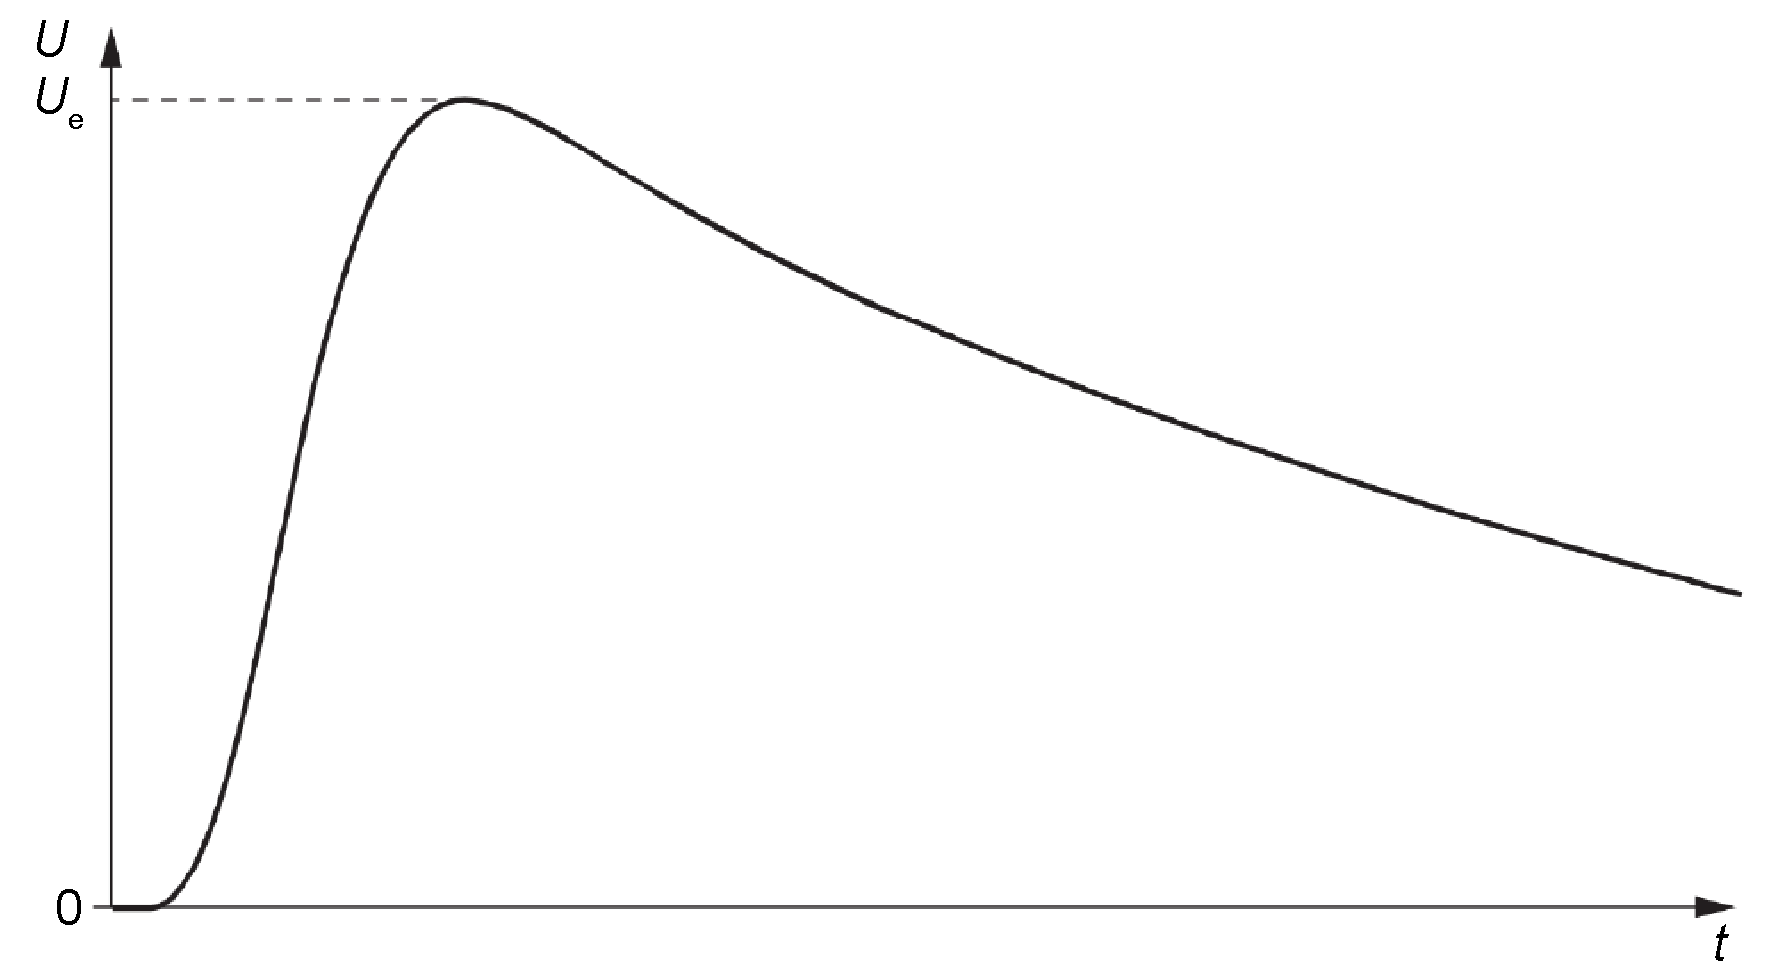
\includegraphics[width=1\textwidth]{img/iec_60060_1_impulso_tension_pleno.png}
    \caption{Impulso de tensión tipo rayo pleno.}
    \label{fig:impulso_tension_pleno}
\end{figure}

\textbf{Sobreelevación / oscilación (overshoot):} Es un incremento de la amplitud de una tensión de impulso debido a una oscilación amortiguada en la cresta, causada por el circuito.

\textbf{Curva registrada:} Es una representación gráfica o digital de los datos de ensayo de una tensión de impulso.
\begin{figure}[H]
    \centering
    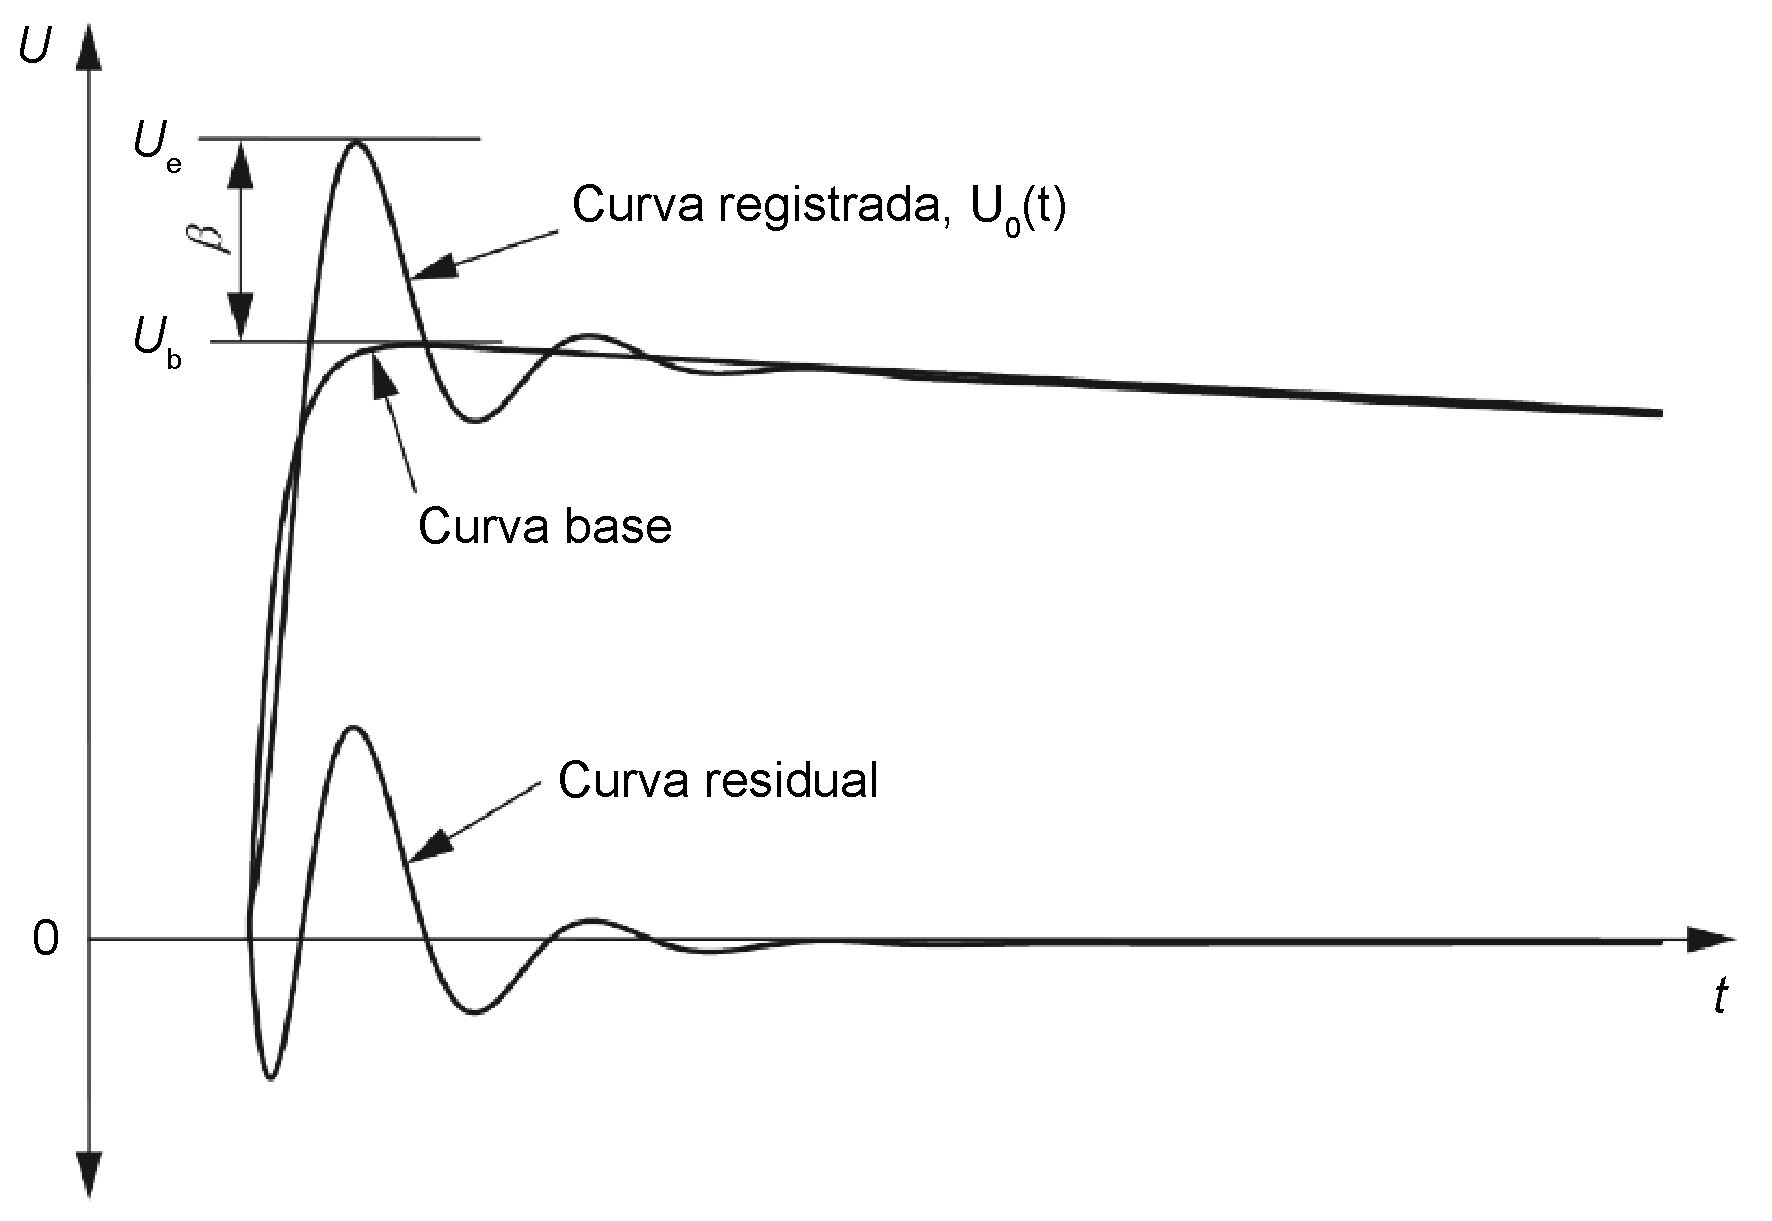
\includegraphics[width=1\textwidth]{img/iec_60060_1_curvas_registro_base_sobreimpulso_residual.png}
    \caption{Curva registrada con sobreimpulso, curva base y curva residual.}
    \label{fig:curvas_registro_base_sobreimpulso_residual}
\end{figure}

\textbf{Nivel de base:} Es el nivel de un registro de un sistema de medición de impulsos cuando hay una entrada cero al instrumento de registro.

\textbf{Curva base $U_\text{m}(t)$:} Es una estimación de una tensión de impulso tipo rayo completa sin una oscilación superpuesta.

\textbf{Curva residual $R(t)$:} Es la diferencia entre la curva registrada y la curva base.

\textbf{Valor extremo $U_\text{e}$:} Es el valor máximo de la curva registrada medido desde el nivel de base en el mismo sentido que el impulso aplicado.

\textbf{Máximo de la curva base $U_\text{b}$:} Es el valor máximo de la curva base.

\textbf{Función de tensión de ensayo:} Es una función de amplitud-frecuencia que se define para representar la respuesta del aislamiento a impulsos con sobreelevación (\emph{overshoot}), dada por la ecuación \ref{eq:func_tension_ensayo}, donde $f$ es la frecuencia en \unit{\mega\hertz}.

\begin{equation}
        k(f) = \frac{1}{1+2,2 \cdot f^2}
        \label{eq:func_tension_ensayo}
\end{equation}
Nota: Aplicar esta función como un filtro paso bajo a la curva de tensión residual, permite el cálculo del valor de la tensión de ensayo de la tensión de impulso tipo rayo completa equivalente.
\begin{figure}[H]
    \centering
    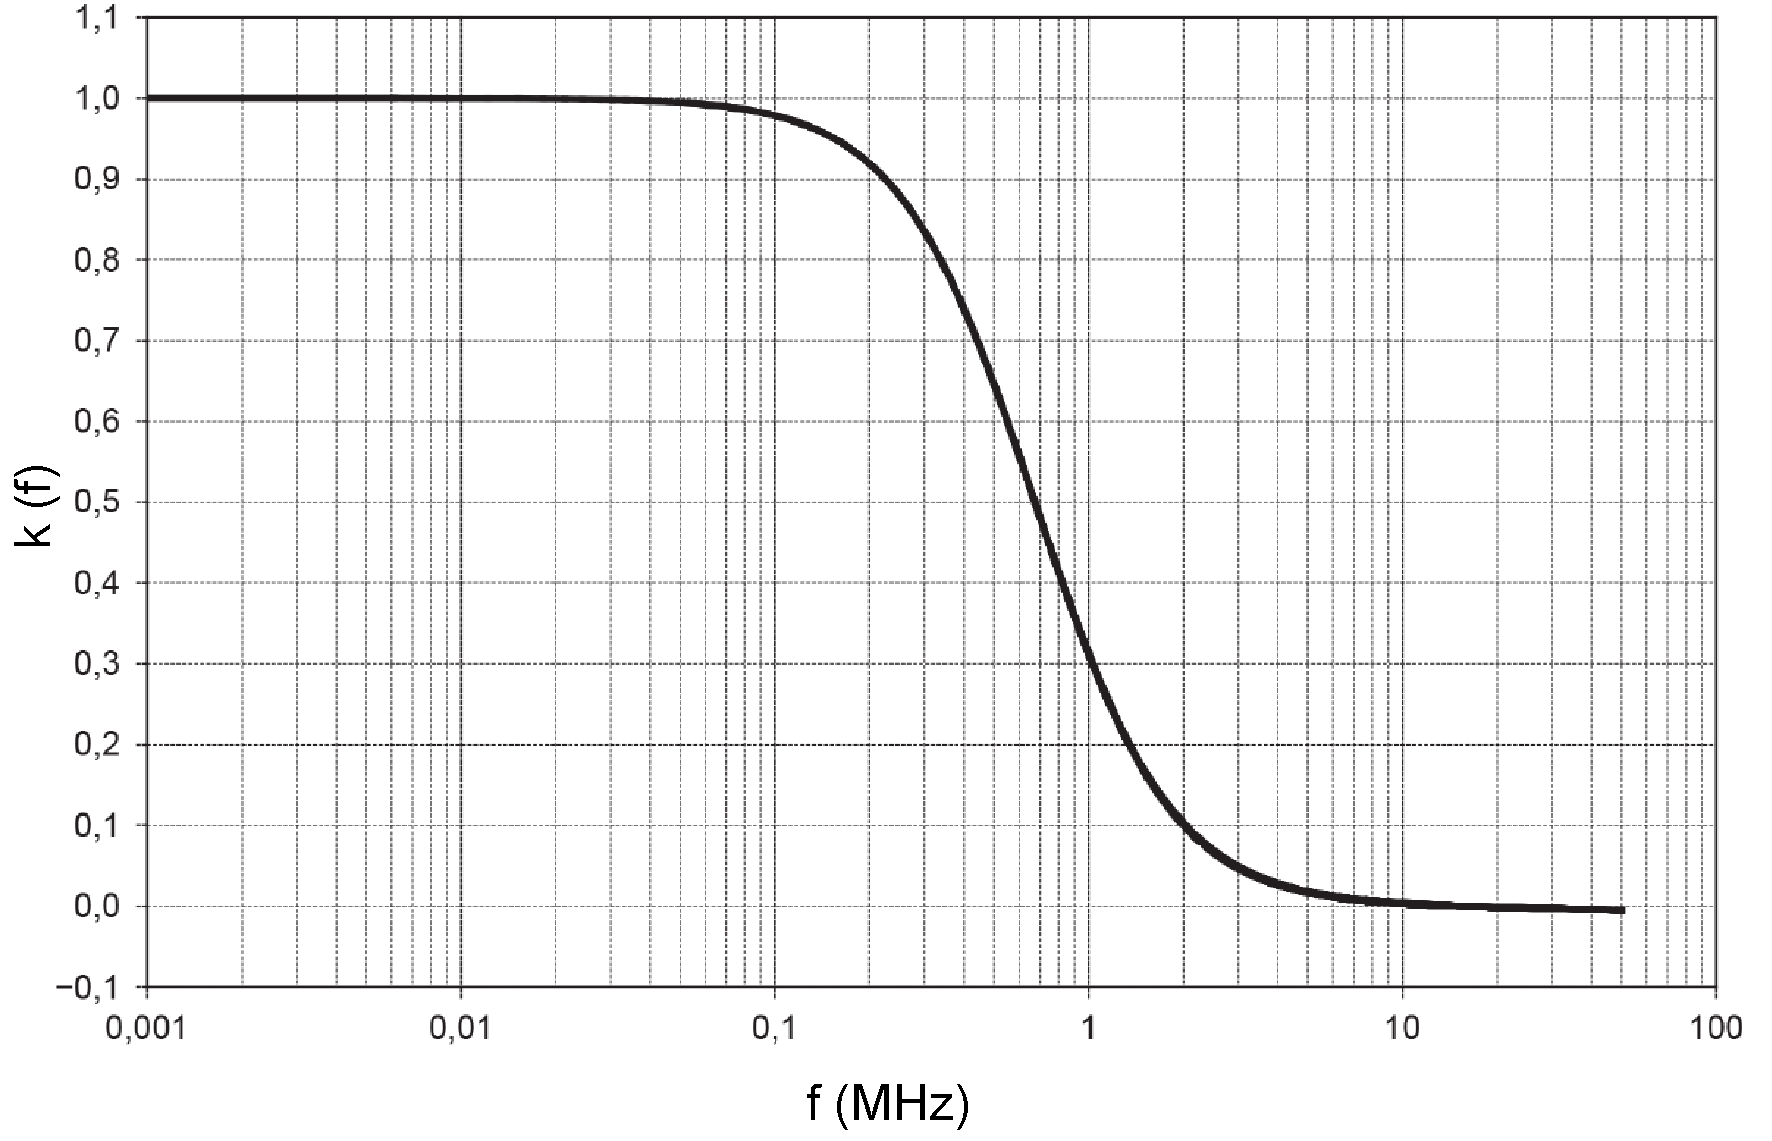
\includegraphics[width=1\textwidth]{img/iec_60060_1_funcion_tension_ensayo.png}
    \caption{Función tensión de ensayo.}
    \label{fig:funcion_tension_ensayo}
\end{figure}

\textbf{Curva residual filtrada ($R_f(t)$):} Es la curva residual filtrada por la función de tensión de ensayo de la ecuación \ref{eq:func_tension_ensayo}.
\begin{figure}[H]
    \centering
    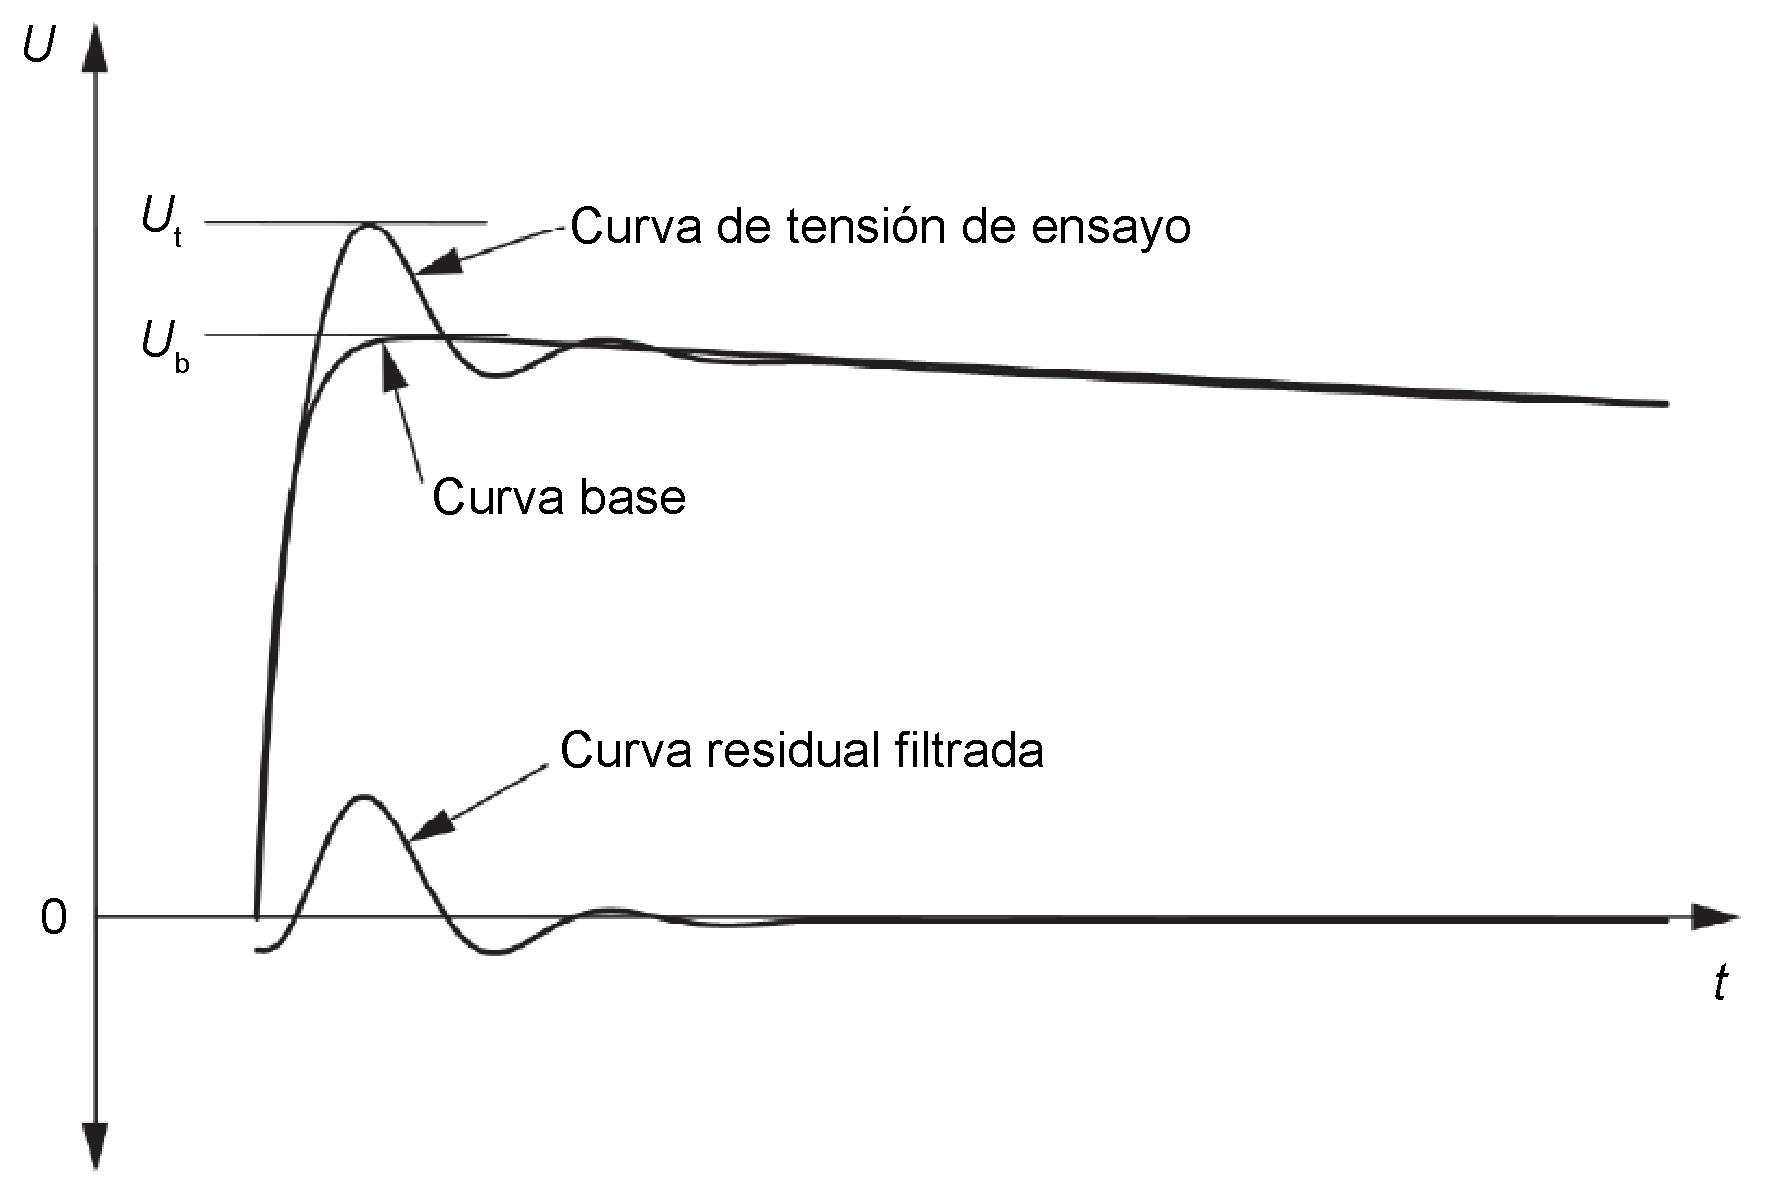
\includegraphics[width=1\textwidth]{img/iec_60060_1_curva_ensayo_base_filtrada.png}
    \caption{Curva tensión de ensayo (suma de curva base y curva residual filtrada).}
    \label{fig:curva_ensayo_base_filtrada}
\end{figure}

\textbf{Curva de tensión de ensayo:} Es la suma de la curva base con la curva residual filtrada. Es una representación matemática del proceso de filtrado y no es una entidad física o un impulso equivalente.
\begin{figure}[H]
    \centering
    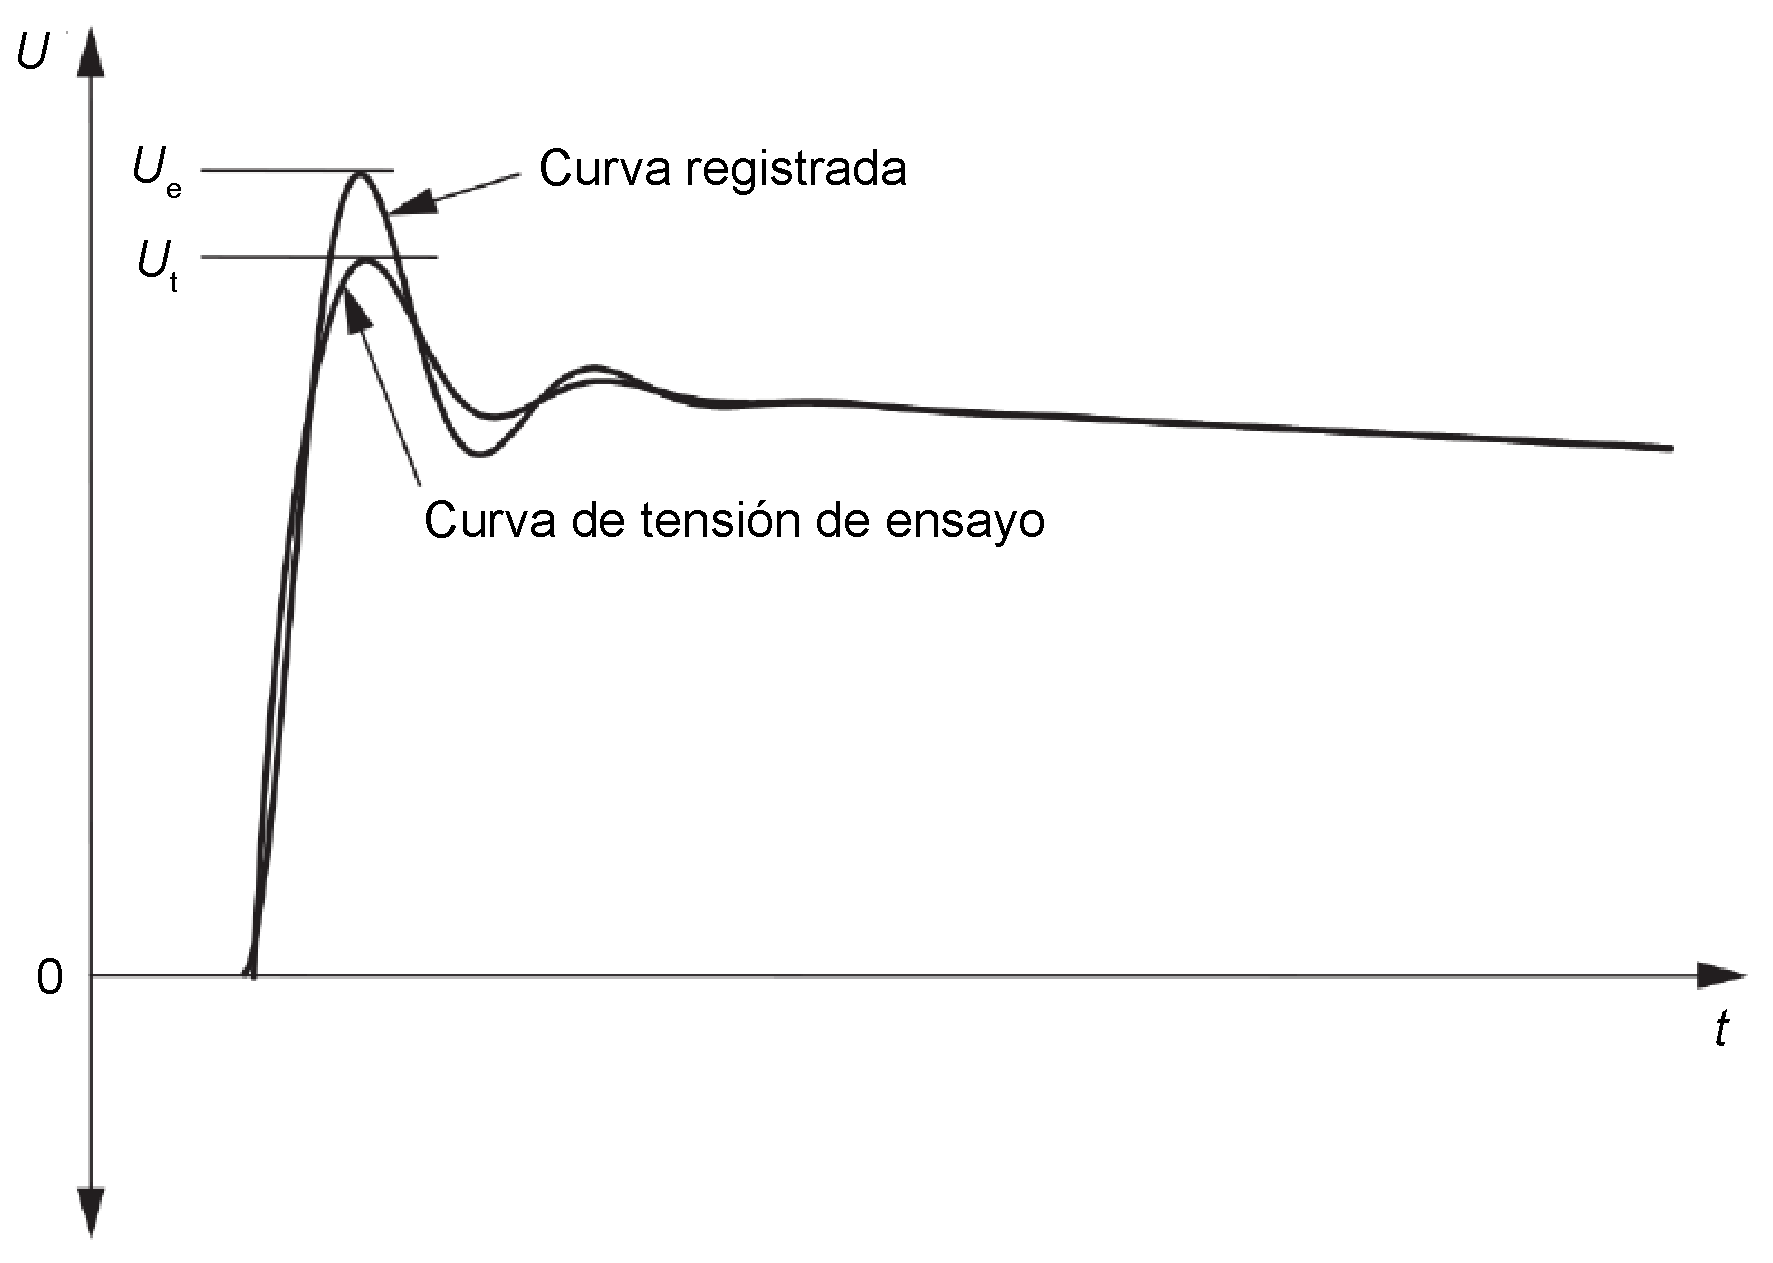
\includegraphics[width=1\textwidth]{img/iec_60060_1_curvas_ensayo_registrada.png}
    \caption{Curva tensión de ensayo y curva registrada.}
    \label{fig:curvas_ensayo_registrada}
\end{figure}

\textbf{Valor de la tensión de ensayo $U_\text{t}$:} Es el valor máximo de la curva de tensión de ensayo, medido desde el nivel de base en el mismo sentido que el impulso aplicado.

\textbf{Magnitud de la sobreelevación $\beta$:} Es la diferencia entre el valor extremo de la curva registrada ($U_\text{e}$) y el valor máximo de la curva base ($U_\text{b}$).

\textbf{Magnitud relativa de la sobreelevación $\beta'$:} Es la relación porcentual entre la magnitud de la sobreelevación y el valor extremo.

\textbf{Tiempo de frente $T_1$:} Es un parámetro virtual definido como $1/0,6$ veces el intervalo $T_{AB}$ entre los instantes en que el impulso es \qty{30}{\percent} y \qty{90}{\percent} del valor de cresta en la curva de tensión de ensayo.

\begin{equation}
    T_1 = \frac{T_{AB}}{0,6} = \frac{t_{90} - t_{30}}{0,6}
    \label{eq:tiempo_frente}
\end{equation}

\begin{figure}[H]
    \centering
    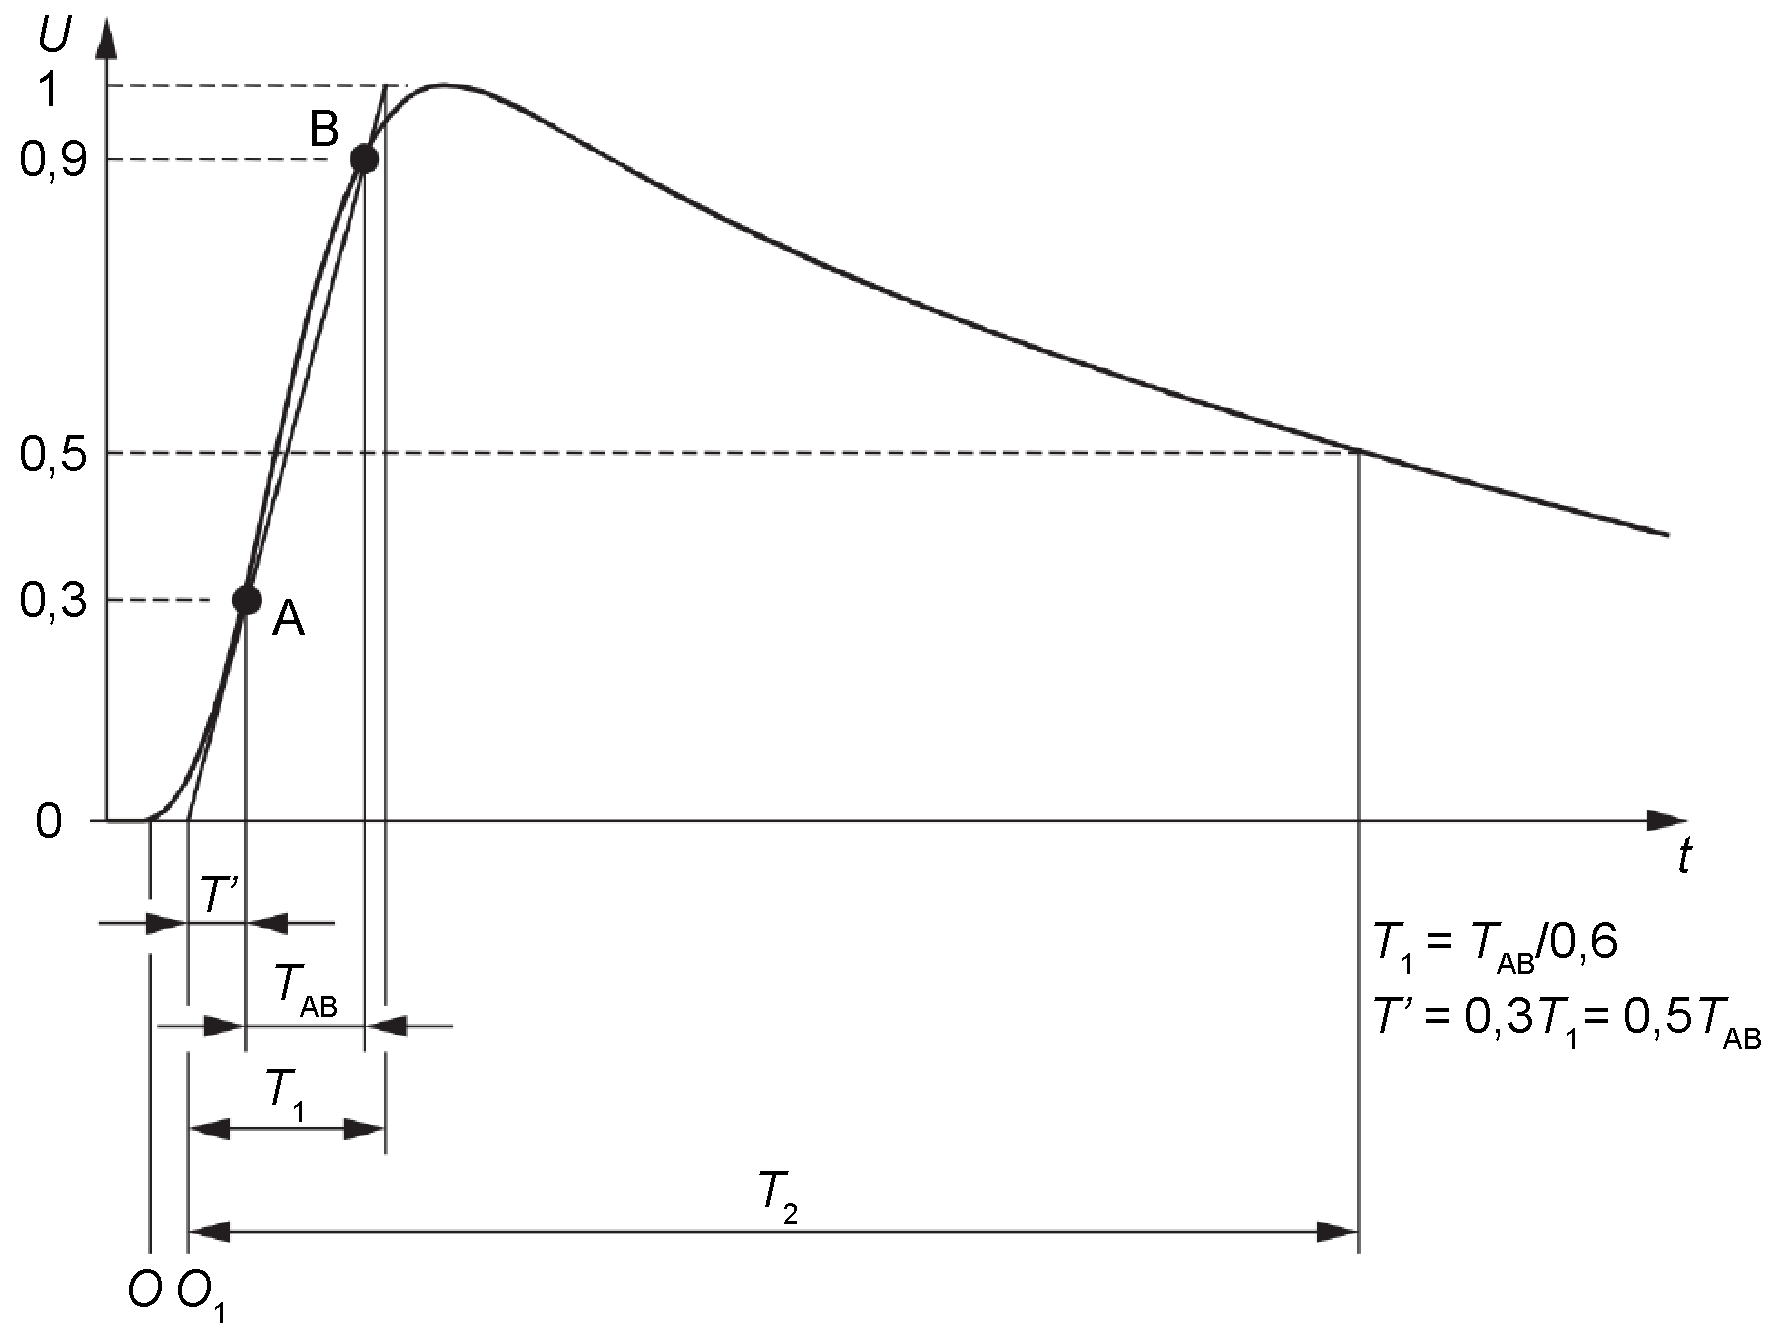
\includegraphics[width=1\textwidth]{img/iec_60060_1_parametros_temporales_impulso_pleno.png}
    \caption{Parámetros de tiempo del impulso de tensión tipo rayo pleno.}
    \label{fig:parametros_temporales_impulso_pleno}
\end{figure}

\textbf{Origen virtual $O_1$:} Es un instante que precede al punto A de la curva de tensión de ensayo en un tiempo $0,3 * T_1$.
\begin{align}
    T' &= 0.5 \cdot T_{AB} \\
    T' &= 0.5 \cdot 0.6 \cdot T_1 \\
    T' &= 0.3 \cdot T_1
    \label{eq:t_prima}
\end{align}
Luego:
\begin{equation}
    O_1 = t_{30} - 0.3 \cdot T_1 = t_{30} - 0.5 \cdot T_{AB}
    \label{eq:origen_virtual}
\end{equation}

\textbf{Tiempo hasta el semi-valor $T_2$:} Es un parámetro virtual definido como el intervalo de tiempo entre el origen virtual ($O_1$), y el instante en que la curva de tensión de ensayo disminuye a la mitad del valor de cresta de la tensión de ensayo ($U_\text{t}$).

\textbf{Tensión de impulso tipo rayo cortada:} Es un impulso tipo rayo que es interrumpido en el frente, cresta o cola por una descarga disruptiva, causando una caída súbita de la tensión.

\textbf{Instante de corte:} Es el instante en el que la extrapolación de la línea entre los puntos del \qty{70}{\percent} y \qty{10}{\percent} (C y D) en el colapso de la tensión cruza el nivel inmediatamente anterior al colapso.
\begin{figure}[H]
    \centering
    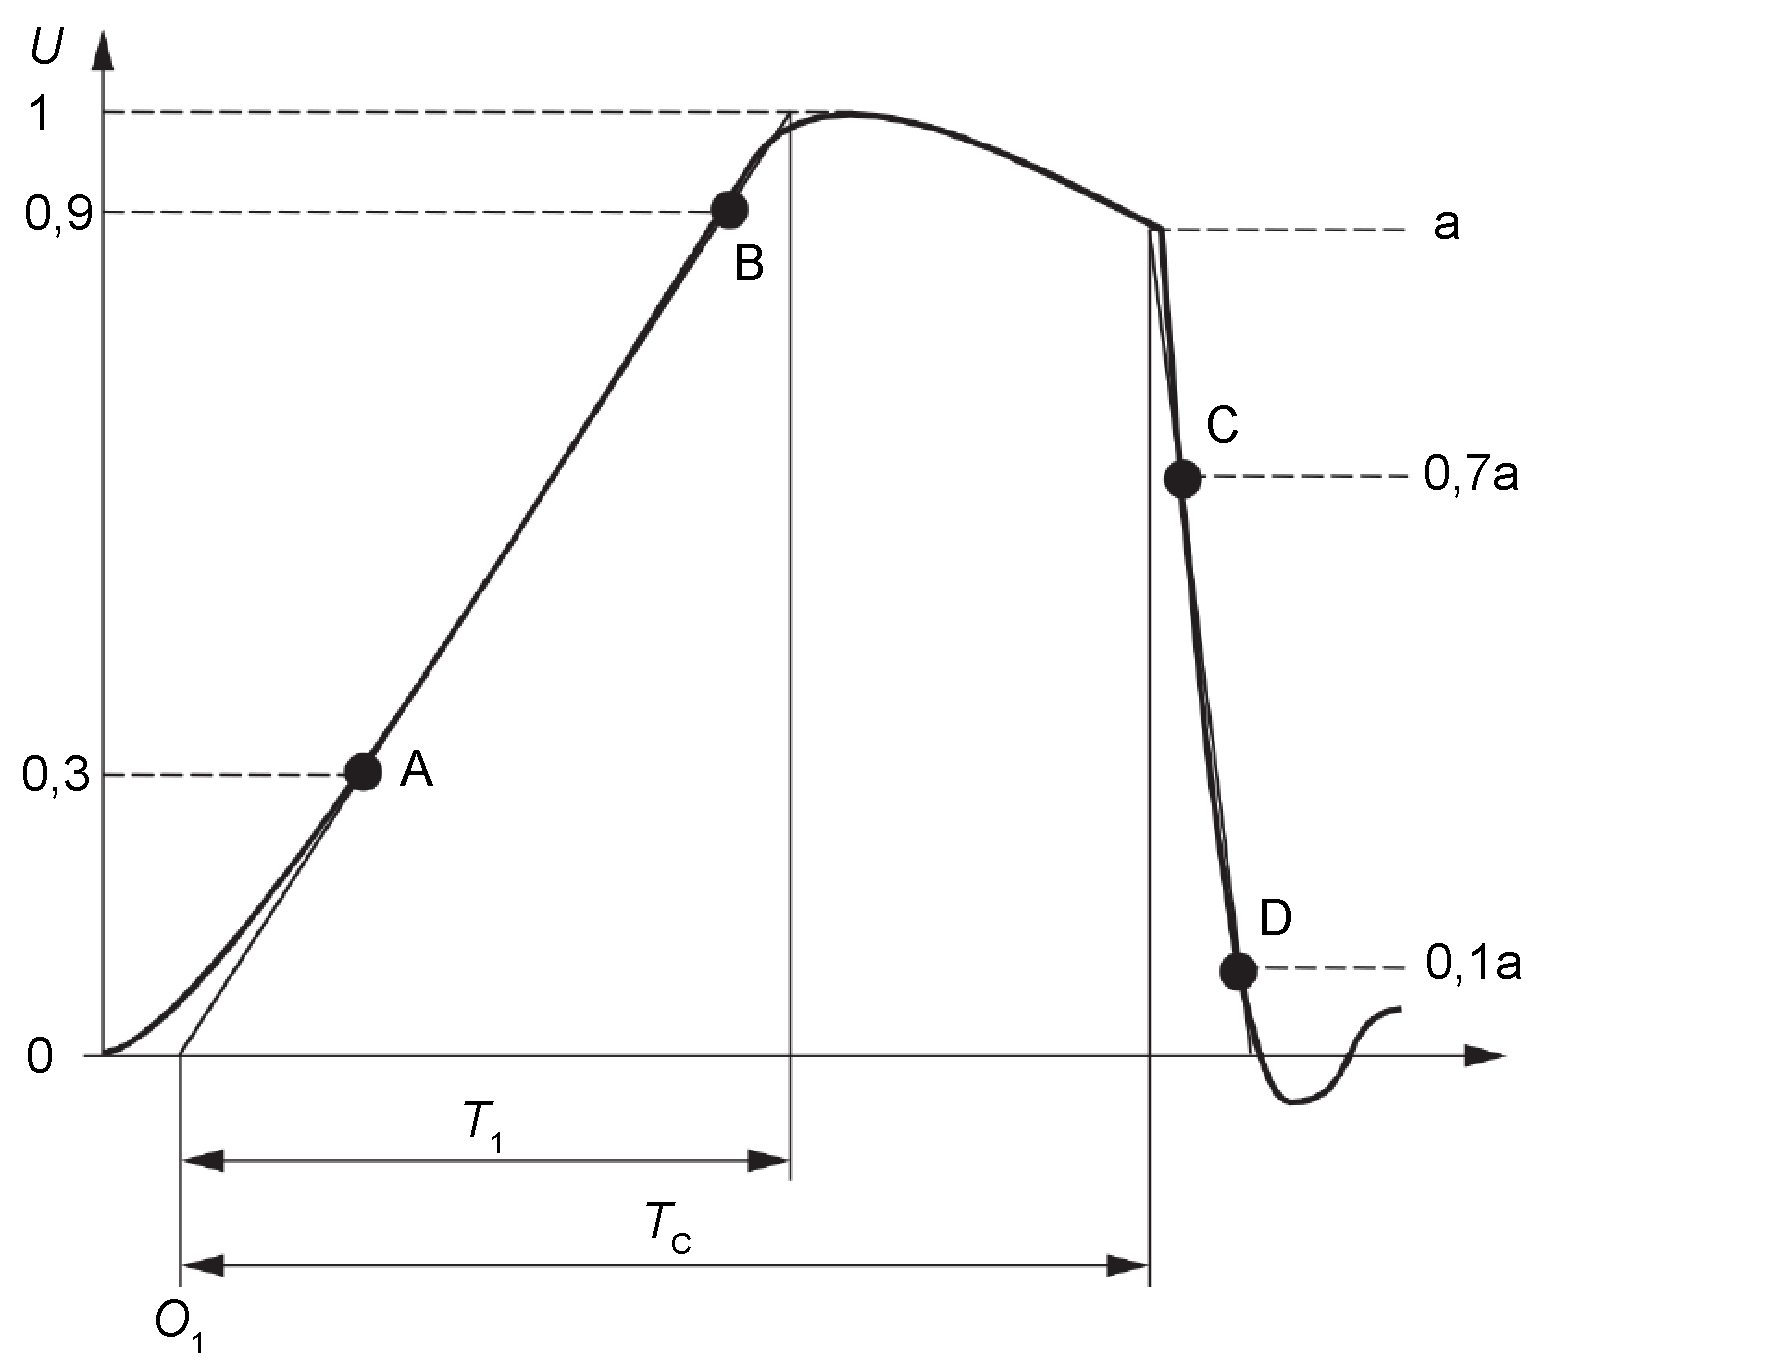
\includegraphics[width=1\textwidth]{img/iec_60060_1_impulso_tension_cortado_cola.png}
    \caption{Impulso de tensión tipo rayo cortado en la cola.}
    \label{fig:impulso_tension_cortado_cola}
\end{figure}

\textbf{Tiempo de corte $T_\text{C}$:} Es el intervalo de tiempo entre el origen virtual ($O_1$) del impulso y el instante relevante.

\subsection{Onda de impulso plena}

Según la norma IEC 60060-1 \cite{iec60060_1}, la tensión de impulso tipo rayo estándar u \enquote{Onda plena} es una tensión de impulso tipo rayo completa y suave, que tiene un tiempo de frente ($T_1$) de \qty{1,2}{\micro\second}, y un tiempo hasta el semi-valor ($T_2$) de \qty{50}{\micro\second}, y se denomina impulso \qty[parse-numbers=false]{1,2/50}{\micro\second}.

Además, la norma establece las tolerancias que acepta en los parámetros característicos, indicados en la tabla \ref{tab:tolerancias_impulso}:

\begin{table}[H]
    \centering
    \caption{Tolerancias de la onda de impulso según IEC 60060-1.}
    \label{tab:tolerancias_impulso}
    \begin{tabular}{@{}ll@{}}
        \toprule
        \textbf{Parámetro}                 & \textbf{Tolerancia}                                                                                     \\ \midrule
        Tensión de ensayo ($U_\text{t}$)   & $\pm \qty{3}{\percent}$                                                                                 \\ \midrule
        Tiempo de frente ($T_1$)           & $\pm \qty{30}{\percent}$                                                                                \\
                                           & y para equipos con $U_\text{m} > \qty{800}{\kilo\volt}$: $\qty{-30}{\percent}$ a $+\qty{100}{\percent}$ \\ \midrule
        Tiempo hasta el semi-valor ($T_2$) & $\pm \qty{20}{\percent}$                                                                                \\ \midrule
        Sobreelevación (OS)                & $\le \qty{10}{\percent}$                                                                                \\ \bottomrule
    \end{tabular}
\end{table}

\subsection{Onda de impulso cortada}

Un impulso tipo rayo estándar cortado u \enquote{Onda cortada}, se denomina así cuando es interrumpido por un entrehierro externo con un tiempo de corte ($T_\text{C}$) entre \qty{2}{\micro\second} y \qty{5}{\micro\second}. Las características del colapso de tensión durante el corte se determinan por el instante del valor \qty{70}{\percent} y \qty{10}{\percent} de la tensión de impulso aplicada antes del colapso.
La duración del colapso de tensión debe ser mucho más rápida que el tiempo de frente ($T_1$) del impulso.

\section{Características del ensayo de impulso}

El ensayo de impulso es una prueba de alta tensión y corta duración, utilizada para verificar la rigidez dieléctrica y el aislamiento de equipos eléctricos, tales como, transformadores, seccionadores y celdas de media tensión, entre otros.

El impulso tipo rayo se produce mediante un generador de impulsos Marx, el cual consiste en un conjunto de capacitores que se cargan en paralelo desde una fuente de tensión continua de baja tensión, que luego se descargan en serie a través del objeto bajo ensayo.

El ensayo de impulso, se realiza aplicando una cierta cantidad de impulsos al objeto bajo ensayo (que dependen de la norma aplicable a dicho elemento), y registrando la respuesta del mismo, mediante un sistema de adquisición de datos, compuesto por un divisor de tensión (resistivo o capacitivo), un atenuador coaxial y un oscilocopio digital.

El análisis de los parámetros del impulso registrado permite evaluar la capacidad del equipo para soportar sobretensiones transitorias referidas a descargas atmosféricas, y determinar su rigidez dieléctrica.

Respecto al análisis de la onda, la norma IEC 60060-1 en su Anexo B, describe un método para el cálculo de los parámetros de las ondas de impulso tipo rayo estándar (plenas y cortadas) con o sin sobreelevación u oscilaciones superpuestas. Este método se basa en la estimación de una curva base, que representa la forma idealizada de un impulso tipo rayo sin oscilaciones, y el cálculo de una curva residual, que representa las oscilaciones superpuestas. Posteriormente, se aplica un filtro a la curva residual, definido por la función de tensión de ensayo (ecuación \ref{eq:func_tension_ensayo}) para luego, obtener la curva de tensión de ensayo, de la cual se calculan los parámetros del impulso. Mientras que, en el Anexo D de la misma norma, contiene una guía de implementación de software para la implementar el ajuste de la curva base, y el filtro digital con la función de tensión de ensayo (ecuación \ref{eq:func_tension_ensayo}).
\newpage
\chapter{Instrumentación y adquisición de señales}
\vspace{3\baselineskip}

Este capítulo detalla los fundamentos teóricos de los sistemas de adquisición de datos en el contexto de ensayos de alta tensión. Se aborda la transición del dominio analógico al digital para la captura de ondas de impulso tipo rayo (\SI[parse-numbers=false]{1,2/50}{\micro\second}) empleando un osciloscopio de almacenamiento digital.

A lo largo de las siguientes secciones, se analizan los conceptos básicos necesarios para entender el funcionamiento de un osciloscopio.

\section{Osciloscopio de almacenamiento digital}

El osciloscopio de almacenamiento digital (DSO, \emph{Digital Storage Oscilloscope}), es un instrumento de medición electrónico, el cual se encarga de convertir la señal analógica a un formato digital, permitiendo su almacenamiento, visualización y posterior análisis.

Su funcionamiento consiste en que la señal ingresa por un circuito analógico de acondicionamiento de entrada, para dirigirse al bloque del convertidor analógico-digital (ADC, \emph{Analog-Digital Converter}) que muestrea y cuantiza la señal a una tasa definida por la base de tiempo. Luego, se almacena la verisón digitalizada en la memoria del osciloscopio, para finalmente presentarla en pantalla.

A continuación, se describen sus parámetros más relevantes, que deben ser considerados al momento de seleccionar el osciloscopio para capturar impulsos de alta tensión.

\textbf{Muestreo de señales:} Consiste en tomar valores de una señal analógica continua a intervalos regulares de tiempo para transformarla en una señal discreta de valores continuos (infinitos valores posibles). La conversión analógica-digital se basa en el teorema de muestreo, el cual establece que la frecuencia de muestreo $(f_s)$ debe ser mayor al doble de la componente de máxima frecuencia $(f_{max})$ presente en la señal, ya que si la velocidad de muestreo es insuficiente, pueden aparecer el fenómeno destructivo del \enquote{aliasing} que muestra erróneamente componentes de frecuencias menores que la señal real, denominadas “Alias”. Matemáticamente, se define:
\begin{equation}
    f_s > 2 f_{max}
\end{equation}

\textbf{Resolución vertical:} La resolución del eje vertical de un osciloscopio está vinculada con la resolución del ADC que tiene internamente, la cual está dada por la cantidad de bits ($N$) del mismo. Consierando que la tensión de entrada varia entre cero y un valor máximo $(V_{max})$, matemáticamente, puede expresarse:
\begin{equation}
    V_{res} = \dfrac{V_{max}}{2^N}
\end{equation}

\textbf{Cuantización de señales:} Consiste de convertir el valor de amplitud continuo en un valor discreto,  dentro de una escala predeterminada. Este proceso introduce un error numérico inherente denominado \textbf{error de cuantización}, ocasionado por la aproximación del valor real al nivel discreto más cercano. El tamaño del paso de cuantización o resolución del LSB (Bit Menos Significativo, por sus siglas en inglés) está dado por:
\begin{equation}
    q = \dfrac{V_{FSR}}{2^N}
\end{equation}
Donde $V_{FSR}$ representa el rango dinámico de escala completa (FSR) (relación entre el valor máximo y el valor mínimo de la señal que se puede capturar o representar), y $N$ es la resolución en bits del convertidor.

\textbf{Longitud de memoria}: El osciloscopio posee una memoria finita ($N_{record}$) para almacenar datos, que junto con la frecuencia de muestreo, determina la ventana de tiempo ($T_{acq}$) que puede registrar datos, a una frecuencia de muestreo ($f_s$) dada.
\begin{equation}
    T_{acq} = \dfrac{N_{record}}{f_s}
\end{equation}

\textbf{Ancho de banda:} Es un parámetro que se mide en \unit{MHz} o \unit{GHz}, e indica la frecuencia máxima a la que puede responder con precisión. Para garantizar una representación fiel de la señal, el ancho de banda debe ser superior a la frecuencia máxima de la señal que se desea medir.

\textbf{Velocidad de muestreo:} Es una medida de la resolución en el tiempo, que se mide en \unit{MSa/s} o \unit{GSa/s}, e indica la cantidad de muestras por unidad de tiempo (normalmente en segundos) que captura el instrumento, por lo tanto, define implícitamente la separación horizontal entre dos muestras consecutivas.

\section{Estándares de comunicación de instrumentos}

En el diseño e implementación de sistemas de instrumentación virtual, la transferencia de los datos desde la memoria del osciloscopio hacia la computadora requiere de interfaces físicas estandarizadas, y protocolos lógicos de control.

Actualmente, la comunicación entre instrumentos de medida y sistemas de adquisición se rige por los siguientes estándares físicos:

\begin{itemize}
    \item \textbf{GPIB (General Purpose Interface Bus / IEEE-488):} Es un estándar de bus de datos digital de corto rango diseñado específicamente para interconectar y controlar dispositivos de prueba y medida, tales como osciloscopios, multímetros y generadores de señal, mediante un controlador central.
    \item \textbf{Comunicaciones Serie (RS-232 y USB):} Los datos resultantes del muestreo y la digitalización suelen transmitirse a la computadora personal empleando el puerto USB o el puerto Serie (utilizando el protocolo RS-232). Estas interfaces son de adopción masiva debido a la arquitectura abierta de las computadoras modernas.
    \item \textbf{LXI (LAN eXtensions for Instrumentation) / Ethernet:} Permite la integración del instrumento en redes de área local, facilitando tasas de transferencia de datos significativamente mayores y posibilitando el control y monitoreo remoto a largas distancias.
\end{itemize}

\subsection{Protocolo VISA}

La diversidad de buses físicos (GPIB, RS-232, USB, Ethernet) presenta un desafío a nivel de desarrollo de software, ya que tradicionalmente cada puerto requería llamadas al sistema y controladores (\emph{drivers}) de bajo nivel completamente distintos. Para mitigar este problema, la industria adoptó la Arquitectura de Software para Instrumentos Virtuales (VISA, \emph{Virtual Instrument Software Architecture}), que funciona como una capa de abstracción de Entrada/Salida, cuyo objetivo es proporcionar una interfaz de software, que encapsula y oculta los detalles de implementación del hardware subyacente. Lo que brinda las siguientes ventajas en el desarrollo de este trabajo:

\begin{itemize}
    \item \textbf{Independencia del bus de hardware:} VISA permite que el software de control envíe comandos al osciloscopio sin necesidad de especificar cómo se gestionan eléctricamente los bits. Si el diseño del sistema migra de una conexión USB a una LAN, el código fuente de control de nivel superior no requiere modificaciones sustanciales.
    \item \textbf{Integración con comandos SCPI:} VISA actúa como el canal de transporte para el protocolo de Comandos Estándar para Instrumentos Programables (SCPI, \emph{Standard Commands for Programmable Instruments}), que es un lenguaje basado en cadenas de texto ASCII estandarizadas (por ejemplo, \texttt{TIMebase:SCALe?}) y los instrumentos interpretan para ajustar sus parámetros como escala de tiempo, resolución vertical, o para entregar el contenido de su memoria hacia la computadora.
    \item \textbf{Gestión de recursos:} La arquitectura asigna descriptores unificados a cada instrumento detectado, centralizando la inicialización, la lectura de las muestras adquiridas, la escritura de comandos de configuración y el cierre de las sesiones de comunicación.
\end{itemize}

Los descriptores de recursos VISA por lo general, tienen la siguiente gramática estructural:
\begin{align*}
    \texttt{Interfaz[Índice]::Dirección\_del\_Dispositivo::[Recurso]}
\end{align*}

\begin{itemize}
    \item \textbf{Interfaz}: Indica el tipo de controlador del puerto.
    \item \textbf{Índice}: Permite diferenciar numéricamente (por ejemplo, el 0 en USB0) cuando existen múltiples tarjetas controladoras del mismo tipo instaladas en la misma computadora (por ejemplo, dos placas PCI para GPIB distintas). Si se omite, VISA asume el valor cero por defecto.
    \item \textbf{Dirección del Dispositivo}: Identificador o ruta simbólica asignada para ubicar de forma unívoca el dispositivo.
    \item \textbf{Recurso}:
    \begin{itemize}
        \item \textbf{\texttt{INSTR}}: La sesión se gestiona utilizando los mecanismos de VISA completos, permitiendo por ejemplo, el uso de comandos de aserción de eventos y de lectura de estado.
        \item \textbf{\texttt{SOCKET}}: VISA actuará simplemente como un puente datos de bajo nivel sin enviar comandos de control propios del protocolo de instrumentación.
    \end{itemize}
\end{itemize}

A continuación, se presentan ejemplos de descriptores de recursos VISA para cada tipo de interfaz física comúnmente utilizada en la adquisición de señales:

\begin{table}[H]
    \centering
    \caption{Ejemplo de descriptor para ASRL (Asynchronous Serial Line)}
    \begin{tabular}{@{}ll@{}}
        \toprule
        \multicolumn{2}{c}{\textbf{\texttt{ASRL1::INSTR}}} \\ \midrule
        \texttt{ASRL1} & Controlador lógico RS-232 o UART.                  \\
                       & Mapeado por el sistema al puerto físico (ej. COM1) \\ \bottomrule
    \end{tabular}
\end{table}

\begin{table}[H]
    \centering
    \caption{Ejemplo de descriptor para USB (Universal Serial Bus)}
    \begin{tabular}{@{}ll@{}}
        \toprule
        \multicolumn{2}{c}{\textbf{\texttt{USB0::0x0957::0x17A6::MY503::INSTR}}} \\ \midrule
        \texttt{USB0}   & Controlador lógico USB. \\
        \texttt{0x0957} & ID del fabricante.      \\
        \texttt{0x17A6} & ID del producto.        \\
        \texttt{MY503}  & Número de serie único.  \\ \bottomrule
    \end{tabular}
\end{table}
%\newpage
\chapter{Procesamiento digital de señales}
\vspace{3\baselineskip}

Este capítulo detalla los fundamentos teóricos del procesamiento digital de señales (DSP). Donde, se describen las técnicas de filtrado digital orientadas a la mitigación de ruido sin alterar la morfología del impulso, y los algoritmos de interpolación necesarios para la extracción de datos, respaldado por la norma IEC 61083-2 \cite{iec61083_2}.

\section{Filtros digitales}

Los filtros digitales son algoritmos matemáticos diseñados para modificar selectivamente las componente en frecuencia de una señal, permitiendo el paso de ciertas frecuencias y atenuando otras, tal como ocurre con los filtros analógicos constituídos por componentes electrónicos (resistencias, capacitores e inductores), ya que buscan simular su comportamiento. Estos se clasifican principalmente en dos grandes familias, FIR o IIR, según la duración de su respuesta al impulso.

\subsection{Filtro de respuesta impulsional finita (FIR)}

Un filtro FIR se caracteriza porque su respuesta al impulso decae a cero en un número finito de pasos. Se implementa mediante una estructura no recursiva, lo que significa que la salida actual del filtro depende exclusivamente de los valores presentes y pasados de la señal de entrada.

Su mayor ventaja es que son intrínsecamente estables, ya que carecen de lazos de retroalimentación que puedan causar oscilaciones.

Tienen desfasaje lineal, lo que asegura que todas las frecuencias de la señal poseen el mismo retraso temporal, logrando fidelidad de la forma de onda original.

Su principal limitación es la ineficiencia computacional. Ya que, para lograr un corte abrupto entre la banda de paso y la de atenuación, necesitan un orden muy elevado, lo cual exige mayor potencia de cálculo.

\subsection{Filtro de respuesta impulsional infinita (IIR)}

Un filtro IIR posee una respuesta al impulso que puede prolongarse indefinidamente en el tiempo.
A diferencia de los FIR, estos filtros utilizan retroalimentación. Es decir, la salida actual se calcula utilizando las entradas actuales y pasadas, y además, las salidas anteriores del propio filtro.

Destacan por su eficiencia computacional. Ya que, pueden lograr caídas de atenuación muy pronunciadas con un orden drásticamente menor que su equivalente en un filtro FIR, lo que los hace ideales para procesamientos muy rápidos en tiempo real o para sistemas con pocos recursos.

Su diseño es más complejo porque son condicionalmente estables, lo que implica que una mala ubicación de sus polos puede provocar que el filtro se vuelva inestable y oscile descontroladamente. Por otro lado, su respuesta de fase es no lineal, lo que introduce una distorsión temporal en la señal, y una distorsión de retardo de grupo en el dominio de la frecuencia, es decir, que distintas componentes en frecuencia de la señal tienen distinto desfasaje, resultado en la alteración de la morfología de la señal de interés.

\subsection{Filtro de fase cero}

El filtrado de fase cero o bidireccional, es una técnica que elimina el desfase temporal antes mencionado, procesando los datos en forma directa e inversa en el dominio del tiempo:
\begin{enumerate}
    \item Se filtra el vector de la señal original $x_1[n]$ en sentido directo, obteniendo $x_2[n]$.
    \item Se invierten las muestras del vector $x_2[n]$, obteniendo $x'_2[n]$.
    \item Se filtra el vector $x'_2[n]$, obteniendo $x_3[n]$.
    \item Se invierten las muestras del vector $x_3[n]$, resultando $x'_3[n]$ alineado en el tiempo con la señal de entrada original $x_1[n]$.
\end{enumerate}

Por lo que, debe considerarse que al pasar dos veces la información por el algoritmo del filtrado, se duplica la atenuación de las frecuencias filtradas, y se duplica de tiempo de cálculo en comparación con un filtrado unidireccional.

\section{Ajuste de curvas e interpolación}

Dado que los datos adquiridos por el osciloscopio, son puntos discretos que representan una señal continua, que posee ruido electromagnético y errores de cuantización. Si bien todos estos fenómenos se pueden atenuar, no se pueden eliminar por completo, por lo tanto, es necesario aplicar técnicas de ajuste de curvas (regresión) para obtener la función que mejor modele el comportamiento de los datos. Mientras que, para obtener los valores ubicados entre dos muestras de la señal discreta, se debe recurrir a la interpolación.

\subsection{Ajuste de curvas (regresión)}

El ajuste de curvas es un proceso matemático que consiste en encontrar la función matemática que mejor represente la tendencia general de una distribución de datos. Su objetivo es minimizar el error global de las predicciones, lo que significa que la curva pasa cerca de los puntos, pero no necesariamente toca alguno de ellos. Este método es especialmente útil cuando los datos no son completamente exactos, presentan dispersión o contienen errores de medición, como ocurre con las señales adquiridas en ensayos eléctricos.

Ahora bien, el tipo de función a ajustar es importante para que represente adecuadamente la morfología del impulso, ya que este método para su ejecución require que se indique una función de base, sin ella no se puede realizar el ajuste porque no se puede evaluar el error al no tener una función de referencia. En este sentido, la norma IEC 60060-1 \cite{iec60060_1} establece que la onda debe ajustarse a una función de doble exponencial (ecuación \ref{eq:doble_exponencial}), para caracterizar adecuadamente el comportamiento del impulso.
\begin{equation}
    u_d(t) = U \cdot \left( e^{-\dfrac{t-t_d}{\tau_1}} - e^{-\dfrac{t-t_d}{\tau_2}} \right)
    \label{eq:doble_exponencial}
\end{equation}

Donde:\\
$u_d(t)$: función de tensión.\\
$t$: tiempo.\\
$U$, $\tau_1$, $\tau_2$ y $t_d$: parámetros a encontrar mediante el ajuste.\\


Para encontrar los parámetros de la función de doble exponencial, se utiliza el \textbf{método de mínimos cuadrados}, que es ampliamente usado en ingeniería para ajustar modelos a datos experimentales.
Este método busca minimizar la suma de los cuadrados de los residuos ($S_r$), que es la distancia vertical entre cada dato observado y el punto correspondiente en la curva calculada. Matemáticamente, esto se expresa como:
\begin{equation}
    S_r = \sum_{i=1}^{N} (y_{i,medicion} - y_{i,modelo})^2
\end{equation}
Donde $y_{i,medicion}$ son los valores registrados, $y_{i,modelo}$ son los valores calculados por el ajuste de curva, y $N$ es el número total de datos observados.

Se utilizan los errores al cuadrado, en lugar de sumar los errores o sus valores absolutos, para evitar que las discrepancias positivas y negativas se cancelen entre sí, y también para asegurar que haya una única solución matemática óptima sin darle un peso desmedido a valores atípicos extremos.

\subsubsection{Tipos de regresión}

La regresión se clasifica principalmente por la relación matemática que hay entre las variables y el modelo:

\textbf{Regresión Lineal Simple:} Los datos muestran una tendencia constante o proporcional, que se ajusta mediante una línea recta.

\textbf{Regresión Polinomial:} Los datos presentan curvatura, ajustándose con polinomios de grado 2 o superior. Aunque generan curvas, se consideran modelos \enquote{lineales por mínimos cuadrados} porque la relación respecto a sus coeficientes desconocidos sigue siendo lineal.

\textbf{Regresión Múltiple:} La variable dependiente está influenciada por dos o más variables independientes.

\textbf{Regresión No Lineal:} Se utiliza para modelos matemáticos complejos que no son lineales con respecto a sus coeficientes, tales como ecuaciones de crecimiento exponencial o potencias.

\subsubsection{Algoritmos de regresión no lineal}
Para resolver los problemas de regresión, especialmente los no lineales, existen diversas técnicas:

\textbf{Linealización:} Es una técnica donde se aplican transformaciones matemáticas (como aplicar logaritmos) a una ecuación no lineal para convertirla en una forma lineal, permitiendo resolverla con los métodos simples de mínimos cuadrados.

\textbf{Métodos de optimización iterativa:} Cuando la ecuación no se puede linealizar, se usan algoritmos numéricos que parten de un valor inicial (semilla) y lo mejoran paso a paso.

Existen muchos algoritmos de optimización, cada uno con sus ventajas y desventajas, pero en este trabajo se adoptó la recomendación de la norma IEC 60060-1 \cite{iec60060_1}, por lo que, se pasa a describir ese modelo directamente, el \textbf{Algoritmo de Levenberg-Marquardt (LM)}. El cual, a su vez, es considerado el estándar de la industria para regresiones no lineales. Es una técnica híbrida donde utiliza un factor de amortiguamiento dinámico (λ), que regula la convergencia, cuando los parámetros están lejos de la solución óptima o si el paso falla y el error aumenta, λ crece obligando al algoritmo a comportarse como el método de \emph{Descenso de Gradiente}, de pasos pequeños, seguros y robusto. Mientras que, a medida que se acerca a la solución, y el error disminuye, λ se hace más pequeño de manera que el algoritmo aproveche la velocidad del método de \emph{Gauss-Newton}. Matemáticamente, esto se expresa como:
\begin{equation}
    w_{i+1} = w_i - \left( J^T J + \lambda diag(J^T J) \right)^{-1} (J^T e)
\end{equation}
Donde:\\
$w_{i+1}$: vector de parámetros actualizado.\\
$w_i$: vector de parámetros actual.\\
$\lambda$: factor de amortiguamiento.\\
$e$: vector de residuos o errores.\\
$J$: matriz Jacobiana, formada por las primeras derivadas parciales de los errores respecto a los parámetros del modelo.\\
$J^T J$: matriz de Hessiana aproximada, compuesta por las segundas derivadas, que modelan la curvatura general de la función de error.\\
$diag(J^T J)$: matriz diagonal. Escala cada parámetro según la curvatura local de la función.\\
$J^T e$: vector gradiente de la función error. Indica la dirección de máxima pendiente.\\

\noindent Si $\boldsymbol{\lambda \rightarrow 0}$, el algoritmo se comporta como el \textbf{Método de Gauss-Newton}, donde asume que la función de error es localmente cuadrática, y utiliza expansiones de series de Taylor para aproximarse al mínimo de forma muy rápida, pero puede ser inestable y fallar si los valores iniciales elegidos están muy lejos del óptimo. Resultando:
\begin{equation}
    w_{i+1} = w_i - \left( J^T J \right)^{-1} (J^T e)
\end{equation}
Si $\boldsymbol{\lambda \rightarrow \infty}$, se comporta como el \textbf{Descenso del gradiente}, que  actualiza los coeficientes moviéndose en la dirección donde el error desciende más rápido. Es muy robusto, es difícil que diverja, pero su convergencia puede ser muy lenta.
\begin{equation}
    w_{i+1} = w_i - \alpha (J^T e)
\end{equation}
Donde:\\
$\alpha$: tamaño de paso de avance de la iteración.

En el metodo de descenso del gradiente $\alpha$ es un escalar, pero en el algoritmo de Levenberg-Marquardt, resulta una matriz diagonal que escala cada parámetro de forma independiente, por lo tanto:
\begin{equation}
    \alpha = diag(J^T J)
\end{equation}

\subsection{Interpolación}

Debido a que, como se indicó antes, los datos adquiridos por el osciloscopio son puntos discretos que representan una señal continua, es necesario aplicar técnicas de interpolación para obtener valores intermedios entre los puntos muestreados. Esto es necesario para encontrar puntos como $U_{30}$ y $U_{90}$, que pueden no coincidir exactamente con los datos de datos adquiridos.

La interpolación polinomial es un proceso matemático que consiste en determinar el único polinomio de grado $n$ que pasa por los $n+1$ puntos de datos conocidos, permitiendo así calcular los valores intermedios. Existen varios métodos de interpolación, cada uno con sus propias características y aplicaciones, entre los más comunes se encuentran:

\textbf{Interpolación Lineal:} Es el método más simple, que conecta dos puntos adyacentes mediante un polinomio de primer grado (una recta). Es rápido pero puede introducir errores significativos si la función subyacente es no lineal con gran curvatura, o si los puntos están muy alejados. Matemáticamente, se puede expresar como:
\begin{equation}
    f_1(x) = f(x_0) + \frac{f(x_1) - f(x_0)}{x_1 - x_0} (x - x_0)
\end{equation}
Donde:\\
$f_1(x)$: polinomio de interpolación de primer grado.\\
$f(x_0)$: punto de origen.\\
$\dfrac{f(x_1) - f(x_0)}{x_1 - x_0}$: pendiente de la recta.\\
$(x - x_0)$: distancia desde el punto de origen hasta el objetivo.

\textbf{Interpolación Polinomial:} Utiliza un polinomio de grado $n$ para pasar por $n+1$ puntos. Puede proporcionar una aproximación más precisa, pero es propenso a oscilaciones si el grado del polinomio es demasiado alto o si los puntos están mal distribuidos. Matemáticamente puede generalizarse como:
\begin{align*}
    f_n(x) &= b_0 + b_1(x - x_0) + b_2(x - x_0)(x - x_1)+ \\
           &+ \ldots + b_n(x - x_0)(x - x_1) \ldots (x - x_{n-1})
\end{align*}
Donde los coeficientes $b_i$ son las diferencias divididas finitas evaluadas a partir de los datos.
\begin{align*}
    b_0 &= f(x_0) \\
    b_1 &= f[x_1, x_0] = \frac{f(x_1) - f(x_0)}{x_1 - x_0} \\
    b_2 &= f[x_2, x_1, x_0] = \frac{\dfrac{f(x_2) - f(x_1)}{x_2 - x_1} - \dfrac{f(x_1) - f(x_0)}{x_1 - x_0}}{x_2 - x_0} \\
    b_n &= f[x_n, \ldots, x_1, x_0] = \frac{f[x_n, \ldots, x_1] - f[x_{n-1}, \ldots, x_0]}{x_n - x_0}
\end{align*}
%\newpage
\chapter{Arquitectura del software y entorno de desarrollo}
\vspace{3\baselineskip}

Este capítulo detalla el diseño estructural del software desarrollado para la adquisición y análisis de ondas de impulso tipo rayo (\SI[parse-numbers=false]{1,2/50}{\micro\second}). Se describe el patrón de diseño implementado para garantizar la escalabilidad y el desacople de los componentes, el flujo de datos desde el osciloscopio digital hasta la generación de reportes, y se presenta la justificación técnica del \emph{stack} de desarrollo seleccionado en contraste con otras alternativas de la industria. Finalmente, se definen los lineamientos de gestión del entorno de desarrollo y el control de versiones aplicados durante el ciclo de vida del proyecto.

\section{Patrones de arquitectura del software}

Actualmente, para el desarrollo de software en general, se existen diversos patrones de diseño que ayudan a organizar el código, mejorar la mantenibilidad y facilitar la escalabilidad. Algunos de los patrones más comunes son:

Modelo-Vista-Controlador (MVC, \emph{Model-View-Controller}): es un patrón de diseño de software que se utiliza para separar la lógica de presentación, la lógica de negocio (procesar los datos, realizar cálculos y tomar decisiones) y la gestión de eventos en una aplicación. En este patrón, el \textbf{Modelo} representa los datos y la lógica de negocio, la \textbf{Vista} se encarga de la presentación visual y la interacción con el usuario, y el \textbf{Controlador} actúa como intermediario entre el Modelo y la Vista, gestionando las entradas del usuario y actualizando la Vista en consecuencia.

Modelo-Vista-Presentador (MVP, \emph{Model-View-Presenter}): es similar al MVC, pero con una separación más clara entre la lógica de presentación y la lógica de negocio. En este patrón, el \textbf{Presentador} se encarga de manejar la lógica de presentación y la interacción con el usuario, mientras que el \textbf{Modelo} sigue representando los datos y la lógica de negocio. La \textbf{Vista} se limita a mostrar los datos proporcionados por el Presentador y a enviar las acciones del usuario al Presentador.

Modelo-Vista-VistaModelo (MVVM, \emph{Model-View-ViewModel}): es una evolución del MVP, el cual introduce el concepto de \textbf{ViewModel}, que actúa como un enlace entre el Modelo y la Vista. En este patrón, el ViewModel expone los datos y comandos que la Vista puede enlazar directamente, lo que facilita la separación de responsabilidades y mejora la testabilidad de la aplicación.


% ===========================================================================================
%\part{MARCO METODOLÓGICO}
%\newpage
\chapter{Implementación del Software}
\vspace{3\baselineskip}

\section{Arquitectura general}
\label{subsec:estructura_arquitectura}

El diseño estructural del software se fundamenta en una separación de responsabilidades, que permite desarrollar y evaluar de forma independiente cada parte del sistema. Con este objetivo, se adoptó el patrón de diseño arquitectónico MVP, el cual divide el sistema en tres capas lógicas bien definidas: la Vista, el Modelo y el Presentador. Esta organización asegura el desacoplamiento de componentes, facilitando la escalabilidad del sistema ante la incorporación de otros modelos de osciloscopios o métodos adicionales de análisis.

La división de tareas facilita la validación algorítmica y control de la incertidumbre matemática especificados en la norma \cite{iec61083_2}, permitiendo someter los algoritmos a ensayos automatizados, aislados de cualquier interfaz gráfica de usuario.

\begin{figure}[H]
    %\centering
    %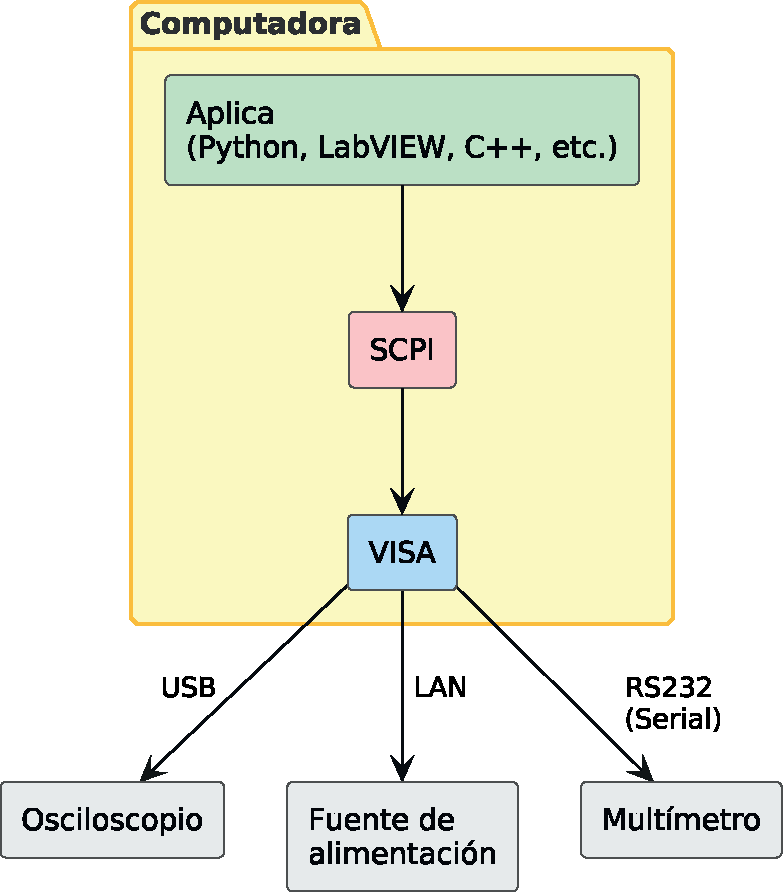
\includegraphics{img/arquitectura_instrumentacion.pdf}
    \caption{Diagrama de bloque de la arquitectura.}
    \label{fig:Lab_1_Circ_1_V1-esquema}
\end{figure}

\subsection{Capa de Presentación: Vista}
\label{subsec:vista}

La \textbf{Vista} maneja de forma exclusiva la representación visual del sistema y la captura de las interacciones del operador. Ya que, solo declara estáticamente la disposición y propiedades de los componentes gráficos.

Esta capa se caracteriza por no tener referencias directas hacia la lógica de adquisición física o los algoritmos de procesamiento digital de señales. Ante cualquier interacción física del usuario, como el accionamiento de botones o la inserción de datos, la Vista emite eventos en forma de señales de Qt (\textbf{Qt Signals}), que son interceptadas por el Presentador para desencadenar el flujo correspondiente.

\subsection{Capa de Lógica y Datos: Modelo}
\label{subsec:modelo}

El \textbf{Modelo} representa el núcleo funcional del software, abarcando el control del instrumental de laboratorio, la lógica de cálculo metrológico y la administración de la persistencia de datos.

Esta capa se subdivide en tres submódulos independientes especializados:

\begin{enumerate}
    \item \textbf{Abstracción de Hardware}: Implementada en el módulo \textbf{GWInstekGDS1000AU}. Encapsula todas las operaciones de control, configuración de canales y adquisición de datos de la memoria del osciloscopio, mediante comandos SCPI, usando el protocolo de comunicación PyVISA.
    \item \textbf{Persistencia y Gestión de Archivos}: Administrada por el módulo \textbf{FileManager}. Maneja la creación y el acceso al sistema de archivos. Su función principal es el almacenamiento en bases de datos utilizando el formato HDF5. Asimismo, gestiona la exportación de resultados a hojas de cálculo tipo CSV o XLSX.
    \item \textbf{Procesamiento Digital de Señales}: Llevado a cabo por el módulo matemático \textbf{LightningImpulseAnalyzer}. Constituye el motor matemático del sistema. Es responsable de acondicionar la señal y extraer sus parámetros característicos según la norma \cite{iec60060_1}.
\end{enumerate}

\subsection{Capa de Coordinación: Presentador}
\label{subsec:presentador}

El \textbf{Presentador}, es implementado en el módulo \textbf{MainPresenter}, y actúa como coordinador de la arquitectura MVP. Tiene como responsabilidad orquestar la interacción entre la interfaz visual y los motores lógico-físicos.

\section{Controlador de \emph{hardware}}
\label{sec:controlador_osciloscopio}

En esta sección se expone la implementación controlador del osciloscopio, cuya función general es abstraer las operaciones de bajo nivel, permitiendo desacoplar la comunicación con el dispositivo del resto del sistema.

\subsection{Interfaz de comunicación y capa de abstracción de hardware}
\label{subsec:interfaz_fisica_hal}

A nivel de \emph{software}, para evitar el acoplamiento directo del código de la aplicación con las llamadas al sistema de bajo nivel (capa física de transmisión), se implementa una Capa de Abstracción de Hardware (HAL, \emph{Hardware Abstraction Layer}), bajo la Arquitectura VISA. Esta capa de abstracción permite que los comandos de consulta (\textit{queries}) y configuración (\textit{writes}) permanezcan independientes de la interfaz de hardware utilizada (sea USB, GPIB, Ethernet o RS-232), permitiendo actualizaciones de la instrumentación sin necesidad de modificar el código del presentador.

El controlador inicializa el administrador de recursos, y ejecuta un escaneo automático para buscar algún dispositivo conectado, que tenga un descriptor de recurso lógico VISA, como el siguiente:
\begin{align*}
    \texttt{ASRL1::INSTR}
\end{align*}

Si encuentra al menos un dispositivo direccionable, se conecta al mismo. La comunicación inicia instanciando el administrador de recursos VISA de Python (PyVISA), acompañado de la biblioteca \texttt{pyvisa-py} para asegurar un entorno multiplataforma sin depender de bibliotecas nativas propietarias.

Sobre el canal de transporte establecido con VISA, el software envía comandos SCPI, que debe cumplir con el siguiente formato indicado en el manual del fabricante \cite{gds1000au_ProgrammingManual}:
\begin{itemize}
    \item \textbf{No sensibilidad a mayúsculas:} Puede usarse mayúsculas y minúsculas.
    \item \textbf{Separación de parámetros:} Al configurar parámetros, debe separarse el comando y su argumento numérico, mediante un carácter de espacio en blanco simple.
    \item \textbf{Finalizador de mensaje:} Cada instrucción enviada al osciloscopio debe finalizar con el carácter delimitador de fin de mensaje \emph{Line Feed} (\textbf{\texttt{LF}}, en hexadecimal \textbf{\texttt{0x0A}} o a la secuencia de escape \textbf{\texttt{\textbackslash n}}), para que el instrumento proceda a interpretar y ejecutar la orden.
\end{itemize}

Para gestionar la configuración del osciloscopio de manera robusta, se implementa una arquitectura, basada en métodos de consulta (\emph{getters}) y configuración (\emph{setters}), que encapsulan los comandos SCPI.

Los métodos de consulta usan la instrucción \textbf{\texttt{.query()}}, reciben una cadena de caracteres, que deben convertir al tipo de dato correspondiente (\texttt{float}, \texttt{int} o \texttt{string}) y la retornan al presentador. En tanto que, los métodos de configuración emplean la instrucción \textbf{\texttt{.write()}}, sin esperar ninguna respuesta del instrumento.

Este flujo se protege con una rutina de control de excepciones que, ante fallos críticos en el bus o pérdidas de sincronismo, aborta la operación y libera los recursos del sistema de forma segura, ya que de lo contrario impediría la reconexión posterior del instrumento, debiendo reiniciar la computadora o el osciloscopio.

A continuación, se ejemplifican los métodos de consulta y configuración de la escala vertical de un canal.
\begin{python}
# Método de consulta.
def get_channel_scale(channel):
    scale = dso.query(f':channel{channel}:scale?')
    v_scale = float(scale)
    return v_scale

# Método de configuración.
def set_channel_scale(channel, value):
    dso.write(f':channel{channel}:scale {value}')
\end{python}

Por otro lado, a nivel físico, la conexión se realiza a través de un puerto USB 2.0 tipo B (esclavo) ubicado en el panel posterior del instrumento, y un puerto USB tipo A (maestro) de la computadora. Aunque, si bien el equipo se conecta a través de un puerto USB, la computadora lo detecta como un dispositivo de comunicación serie virtual\footnote{El controlador (\emph{driver}) USB, está disponible en la página del fabricante \cite{gds1000au_driver}.}, bajo la Clase de Dispositivo de Comunicación con Modelo de Control Abstracto (CDC-ACM, \emph{Communication Device Class - Abstract Control Model}), que aparece en el administrador de dispositivos con el siguiente nombre \cite{gds1000au_ProgrammingManual}:
\begin{align*}
    \texttt{COM1}
\end{align*}
Donde \texttt{COM1} identifica el número de puerto serie virtual asignado por el sistema operativo.

\subsection{Sistema de Adquisición y Almacenamiento}
\label{subsec:arquitectura_flujo}

La adquisición del impulso de alta tensión desde el generador Marx, hasta el almacenamiento en la computadora, se estructuran de la siguiente forma:

\begin{enumerate}
    \item Acondicionamiento analógico.
    \item Captura de impulso
    \item Digitalización.
    \item Desempaquetado de datos.
    \item Reconstrucción y escalamiento de la onda.
\end{enumerate}

\subsubsection{Acondicionamiento analógico}

La señal eléctrica, debe ser adaptada en amplitud antes de ingresar al osciloscopio, para no dañarlo.

Para el canal de tensión (CH1), la señal se deriva utilizando un divisor de tensión resistivo, acoplado en cascada serie con un atenuador coaxial, por lo que el factor de atenuación equivalente resulta:
\begin{equation}
    \label{eq:atenuacion_tension}
    A_{\text{CH1}} = \text{Divisor} \times \text{Atenuador}
\end{equation}

Para el canal de corriente (CH2), la descarga atraviesa una resistencia shunt conectada en serie con el elemento bajo ensayo, de la cual se toma su tensión a bornes, acoplada a un atenuador que reduce su magnitud a niveles adecuados.
\begin{equation}
    \label{eq:atenuacion_corriente}
    A_{\text{CH2}} = R_\text{Shunt} \times \text{Atenuador}
\end{equation}

Ambas señales llegan al instrumento por medio de cables coaxiales de \qty{50}{\ohm}, para reducir acoplamientos electromagnéticos parásitos (EMI).

\subsubsection{Captura de impulso}
\label{subsec:captura_impulso}

La captura de impulsos (\qty[parse-numbers=false]{1.2/50}{\micro\second}) requiere que el osciloscopio opere en modo de disparo único (\emph{Single Trigger}), dado que es un transitorio no periódico.

Cuando el operador inicia el modo de captura desde la GUI, el presentador crea y ejecuta un subproceso asíncrono, que mediante el controlador de \emph{hardware}, realiza un sondeo periódico (\emph{polling}) al osciloscopio, para saber el estado de disparo del mismo.

Al detectar el impulso finaliza el bucle de \emph{polling} y emite una señal, que es capturada en el hilo de ejecución principal por un receptor (\emph{slot}) del presentador, y finaliza el subproceso.

Como el instante de descarga es indeterminado, se implementa un hilo de ejecución secundario asíncrono, dedicado a consultar el estado de disparo, ya que si se ejecutara en el hilo principal, sería una operación bloqueante, que congele la aplicación e inhabilite la GUI. Por lo que, así se mantiene siempre reactivo el hilo principal de eventos gráficos, permitiendo al usuario manipular oscilogramas previos, cargar campos o cualquier otra acción, mientras el sistema espera la captura del impulso.

\subsubsection{Digitalización}

Las señales eléctricas que ingresan a los bornes analógicos del osciloscopio, se muestrean a una tasa que depende de la base de tiempo utilizada. Después, el convertidor analógico-digital (ADC) realiza la cuantización en amplitud, dividiendo el rango dinámico vertical en $2^8 = 256$ niveles de tensión discretos (\num{8} bits). A continuación, se graban en la memoria del instrumento.

\subsubsection{Desempaquetado de datos}
\label{subsec:desempaquetado_datos}

Luego de que el osciloscopio digitalice la señal, el presentador ordena la descarga de los datos brutos (\emph{RAW}) de los canales habilitados, y recibe un bloque de datos, compuestos por el encabezado y el vector de datos de la onda, que cumple con la siguiente estructura\footnote{La estructura de datos descrita en el manual del fabricante tiene algunas diferencias con los resultados obtenidos del instrumento, debido a la dificultad que esto presentó al momento de intentar procesarla, se contactó con el frabricante obteniendo un script de procesamiento del paquete de datos, que se corresponde con el formato indicado en este trabajo. A su vez, se encontró que el manual de programación de la series GDS-1000B aporta detalles explicativos sobre cómo procesar esta estructura \cite{gds1000b_ProgrammingManual}} \cite{gds1000au_ProgrammingManual}:

\begin{equation*}\label{eq:formato_memoria}
\text{\texttt{\# A B C D E}}
\end{equation*}
\begin{enumerate}
    \item[\texttt{\#:}] [\num{1} byte] Caracter ASCII que indica el inicio de la cabecera.
    \item[\texttt{A:}] [\num{1} byte] Dígito ASCII que especifica la cantidad de caracteres que componen el campo \texttt{B}. Para adquisiciones estándar toma el valor ASCII \texttt{'4'}, mientras que para adquisiciones de memoria extendida toma el valor \texttt{'7'}.
    \item[\texttt{B:}] [\num{4} o \num{7} bytes] Cadena de caracteres ASCII que representa el tamaño total en bytes del bloque de datos que le sigue (\texttt{C}+\texttt{D}+\texttt{E}).
    Para adquisiciones estándar toma el valor ASCII \texttt{'8008'}, mientras que para adquisiciones de memoria extendida puede tomar los valores \texttt{'2000008'} o \texttt{'4000008'}.
    \item[\texttt{C:}] [\num{4} bytes] Intervalo de tiempo ($\Delta t$) entre dos muestras consecutivas de la señal, en formato de punto flotante de precisión simple según IEEE-754 (\num{32} bits), en orden \emph{little-endian} (se envía primero el byte menos significativo):
    \begin{equation*}\label{eq:periodo_muestreo}
    \Delta t = t[n+1] - t[n]
    \end{equation*}
    \item[\texttt{D:}] [\num{4} bytes] Bloque de datos no utilizado.
    \item[\texttt{E:}] [\num{8e3}, \num{2e6} o \num{4e6} bytes] Vector de datos de la onda, cuya longitud es definida en el campo \texttt{B}. Cada valor entero (base \num{10}) es expresado con \num{2} bytes (\num{16} bits), y transmitidos en orden \emph{big-endian} (se envía primero el byte más significativo).
\end{enumerate}

Una vez finalizada la descarga de datos, el presentador ordena al controlador de \emph{hardware} que decodifique cada bloque acorde a su formato, considerando la estructura recién mencionada.

\subsubsection{Reconstrucción y escalamiento de la onda}

Con el vector de valores enteros brutos decodificado, primero se aplica la ecuación \eqref{eq:reconstruccion_tension} para reconstruir la forma de onda que llegó a bornes del osciloscopio, considerando la escala vertical configurada al momento de la captura, y el Factor AD = \num{25} definido en el manual de programación del fabricante \cite{gds1000au_ProgrammingManual}:
\begin{equation}
\label{eq:reconstruccion_tension}
\text{Onda sin escalar}[n] = \text{Datos brutos}[n] \times \frac{{\text{V/div}}}{\text{Factor AD}}
\end{equation}
A continuación, para obtener las magnitudes reales aplicadas al objeto bajo ensayo, se multiplica escalarmente los vectores de tensión y corriente, por sus respectivos factores de atenuación, cargados por el usuario en los campos pertinentes de la ventana, aplicando la siguiente ecuación:
\begin{equation}
\label{eq:reconstruccion_tension_total}
{\text{Onda escalada}}[n] = \text{Onda sin escalar}[n] \times A_{\text{CH<X>}}
\end{equation}
Los vectores resultantes de tensión (en volts, \unit{\volt}) y de corriente (en amperes, \unit{\ampere}), se transfieren al módulo de procesamiento matemático para determinar sus parámetros normativos: tiempo de frente $T_1$, tiempo de cola $T_2$, valor de cresta $U_{\text{t}}$ y sobreimpulso OS, conforme a los requerimientos de la norma \cite{iec60060_1}.

\section{Motor de Cálculo: Procesamiento de Señales y Ajuste de Curvas}
\label{sec:motor_calculo}

Este componente constituye el núcleo matemático del software, y es responsable de obtener los parámetros normativos a partir de los arreglos temporales de tensiones discretas adquiridas por el \emph{hardware}.

El motor de cálculo ha sido diseñado exclusivamente para cumplir con las normas IEC 60060-1 \cite{iec60060_1} e IEC 61083-2-1 \cite{iec61083_2}, aplicando criterios de modularidad, que permiten su validación automatizada e independiente del resto de la aplicación.

\subsection{Flujo algorítmico de cálculo}
\label{sec:flujo_algoritmico}

Este proceso se divide en tres fases operativas: preprocesamiento común, clasificación dinámica y reconstrucción de la señal.

\subsubsection{Fase I: Acondicionamiento Inicial}

Esta etapa es común a todos los registros adquiridos.
\begin{enumerate}
    \item \textbf{Eliminación de offset}: Se calcula el valor de tensión continua ($V_{\text{offset}}$) promediando estadísticamente una ventana de datos adquiridos ($N_{\text{pretrigger}}$) en el instante previo al disparo (``pre-trigger''), donde la curva registrada ($U_\text{e}[n]$) es nula.
    \begin{equation}
        \label{eq:calculo_offset}
        V_{\text{offset}} = \frac{1}{N_{\text{pretrigger}}} \sum_{n=1}^{N_{\text{pretrigger}}} U_\text{e}[n]
    \end{equation}
    El vector de tensión corregida se calcula como:
    \begin{equation}
        \label{eq:eliminacion_offset}
        U_{\text{corregida}}[n] = U_\text{e}[n] - V_{\text{offset}}
    \end{equation}
    \item \textbf{Normalización de polaridad}: Dado que los impulsos pueden ser de polaridad positiva o negativa, el algoritmo detecta el sentido del impulso evaluando el signo de la muestra extrema:
    \begin{equation}
        \label{eq:buscar_polaridad}
        \text{polaridad} = \text{sign}(\text{arg max} |U_{\text{corregida}}[n]|)
    \end{equation}
    El vector de tensión corregida se multiplica por este término para simplificar el resto del procesamiento, asegurando que el análisis sea exclusivamente en el semiplano positivo:
    \begin{equation}
        \label{eq:normalizacion_polaridad}
        U_{\text{abs}}[n] = \text{polaridad} \cdot U_{\text{corregida}}[n]
    \end{equation}
    \item \textbf{Normalización unitaria}: Se normaliza la amplitud al dominio unitario respecto a su valor de cresta.
    \begin{equation}
        \label{eq:onda_normalizada}
        U_{\text{norm}}[n] = \frac{U_{\text{abs}}[n]}{\max(U_{\text{abs}}[n])}
    \end{equation}
\end{enumerate}

\subsubsection{Fase II: Bifurcación de análisis e identificación de parámetros base}

En este punto, el flujo se divide según si debe procesar un impulso de referencia (pleno) o un impulso de ensayo, que puede ser pleno o cortado.

\textbf{Caso A: Análisis de impulso de referencia (pleno)}

Se asume que la onda es plena y se procede al ajuste paramétrico.
\begin{enumerate}[resume]
    \item \textbf{Segmentación de datos}: Se selecciona una ventana de datos en el intervalo comprendido entre el \qty{20}{\percent} en el flanco de subida y el \qty{40}{\percent} en la cola de descarga del impulso.
    \item \textbf{Ajuste de curva base}: Se realiza un ajuste paramétrico no lineal sobre la ventana de muestras, utilizando el algoritmo de \textbf{Levenberg-Marquardt}, teniendo como modelo de estimación la función de doble exponencial:
    \begin{equation}
        \label{eq:modelo_doble_exponencial}
        u_d[n] = U \cdot \left( e^{-\frac{t - t_d}{\tau_1}} - e^{-\frac{t - t_d}{\tau_2}} \right)
    \end{equation}
    Donde los coeficientes desconocidos a determinar son:
    \begin{itemize}
        \item $U$ el parámetro de amplitud escalar.
        \item $\tau_1$ la constante de tiempo de descarga.
        \item $\tau_2$ la constante de tiempo de carga.
        \item $t_d$ el retardo temporal del origen virtual.
    \end{itemize}
\end{enumerate}

\textbf{Caso B: Análisis de ensayo (LI vs. LIC)}

Si evalúa una onda de ensayo, se inyectan los parámetros de la onda de referencia procesada en el \textbf{Caso A}, y se ejecuta el siguiente análisis:
\begin{enumerate}[resume]
    \item \textbf{Cálculo del desfasaje temporal}: El corrimiento temporal, $t_L$, entre el frente de onda del último impulso con el de referencia, se calcula como el promedio de las diferencias de los instantes de tiempo, correspondientes al \qty{30}{\percent}, \qty{50}{\percent} y \qty{80}{\percent} de $U_\text{t}$ respectivamente, de ambos impulsos.
    \begin{equation}
        t_L = \frac{\left( t_{30, \text{ref}} - t_{30, \text{i}} \right) + \left( t_{50, \text{ref}} - t_{50, \text{i}} \right) + \left( t_{80, \text{ref}} - t_{80, \text{i}} \right)}{3} 
    \end{equation}
    \item \textbf{Alineación del eje temporal}: Se obtiene el vector temporal alineado del impulso de ensayo, $t_\text{aligned}[n]$, partiendo de su vector temporal original $t[n]$, al que se lo desplaza la cantidad $t_L$.
    \begin{equation}
        \label{eq:eje_alineado}
        t_\text{aligned}[n] = t[n] + t_L
    \end{equation}
    \item \textbf{Clasificación del impulso}: Se calcula la diferencia absoluta punto a punto entre el impulso de ensayo y el de referencia, usando sus vectores normalizados en amplitud.
    \begin{equation}
        \label{eq:umbral_desviacion}
        | U_{\text{norm, i}}[n] - U_{\text{norm, ref}}[n] | > umbral
    \end{equation}
\end{enumerate}

En caso de que la desviación no supere el umbral, la onda es clasificada como \textbf{impulso pleno (LI)} y el flujo se dirige al \textbf{Caso A}.

Si la desviación supera el umbral, la onda se clasifica como \textbf{impulso cortado (LIC)} y se procede a analizar el colapso de la onda.
\begin{enumerate}[resume]
    \item \textbf{Cálculo del factor de escala}: Se calcula como el promedio del intervalo comprendido entre el \qty{30}{\percent} y \qty{80}{\percent} de $U_{\text{corregida}}[n]$ del frente de la onda de ensayo y la de referencia.
    \begin{equation}
        \overline{U_\text{i}} = \frac{1}{N} \sum_{n = k_{30\%}}^{k_{80\%}} U_\text{i}[n]
    \end{equation}
    \begin{equation}
        \overline{U_\text{ref}} = \frac{1}{N} \sum_{n = k_{30\%}}^{k_{80\%}} U_\text{ref}[n]
    \end{equation}
    \begin{equation}
        \label{eq:factor_escala_e}
        E = \frac{\overline{U_\text{i}}}{\overline{U_\text{ref}}}
    \end{equation}
    \item \textbf{Escalado de la curva base}: Debido a que la descarga disruptiva hace colapsar el ajuste por el corte abrupto de la señal, se sintetiza la curva base de la onda de referencia $U_\text{b, ref}[n]$, y se escala en amplitud con el factor de escala $E$.
    \begin{equation}
        \label{eq:curva_base_lic}
        U_\text{b, i}[n] = E \cdot U_\text{b, ref}[n]
    \end{equation}
    \item \textbf{Tiempo de corte}: Se analiza la cola del impulso, minimizando la derivada primera para localizar el sector de máxima pendiente de caída:
    \begin{equation}
        \label{eq:gradiente_colapso}
        n_\text{abrupto} = \text{arg min}\left(\frac{\text{d} U_{\text{cola}}[n]}{\text{d} t}\right)
    \end{equation}
    El inicio del colapso se encuentra evaluando el punto de inflexión local mediante la derivada segunda:
    \begin{equation}
        \label{eq:punto_inflexión}
        n_\text{inflexion} = \text{arg min}\left(\frac{\text{d}^2 U_\text{cola}[n]}{\text{d}^2 t}\right)
    \end{equation}
    Con ese índice se obtiene la tensión del colapso:
    \begin{equation}
        U_\text{colapso} = U_\text{corregida}[n_\text{pico} + n_\text{inflexion}]
    \end{equation}
    Se calculan los instantes correspondientes al \qty{70}{\percent} y al \qty{10}{\percent} de $U_\text{colapso}$ sobre el flanco descendente, para extrapolar linealmente el instante de corte, para el nivel de $U_{\text{colapso}}$:
    \begin{equation}
        t_c = t_{70} + (U_{\text{colapso}} - U_{70}) \left(\frac{t_{10} - t_{70}}{U_{10} - U_{70}}\right)
    \end{equation}
    Finalmente, se calcula el tiempo de corte respecto al origen virtual:
    \begin{equation}
        T_c = t_c - O_1
    \end{equation}
\end{enumerate}

\subsubsection{Fase III: Convergencia, Filtrado y Parámetros Característicos}

Independientemente de la ruta ejecutada en la Fase II, el algoritmo converge obteniendo una curva registrada y una curva base (ajustada numéricamente o escalada analíticamente), para avanzar a la secuencia final:
\begin{enumerate}[resume]
    \item \textbf{Cálculo de curva residual}: Se obtiene como la diferencia algebraica entre la curva corregida ($U_{\text{corregida}}[n]$) y la curva base ($U_\text{b}[n]$) construída con los parámetros obtenidos del ajuste:
    \begin{equation}
        \label{eq:curva_residual}
        R[n] = U_{\text{corregida}}[n] - U_\text{b}[n]
    \end{equation}
    \item \textbf{Filtrado digital de fase cero}: 
    Se obtiene la curva residual filtrada ($R_f[n]$), aplicando un filtro digital IIR a la curva residual ($R[n]$). Para reducir el ruido de muy alta frecuencia relacionado a la interferencia electromagnética, sin perder oscilaciones propias del ensayo.
    \item \textbf{Curva de tensión de ensayo}: Se sintetiza la curva de ensayo ($U_\text{t}[n]$) sumando algebraicamente la curva base analítica con la residual filtrada:
    \begin{equation}
        \label{eq:curva_ensayo}
        U_\text{t}[n] = U_\text{b}[n] + R_f[n]
    \end{equation}
    \item \textbf{Cálculo de parámetros característicos}: A partir de la curva de tensión de ensayo $U_\text{t}[n]$, se calculan los parámetros normativos. Dado que la señal procesada es de tiempo discreto, hay valores analíticos que pueden no corresponder con las muestras obtenidas, por lo que para encontrarlos se realiza una interpolación lineal.
    \begin{itemize}
        \item \textbf{Valor de cresta} ($U_\text{t}$): Es la amplitud máxima de la curva de tensión de ensayo $U_\text{t}[n]$:
        \begin{equation}
            \label{eq:valor_cresta}
            U_\text{t} = \text{max}(U_\text{t}[n])
        \end{equation}
        \item \textbf{Tiempo de frente} ($T_1$): Se calcula como el cociente del intervalo temporal transcurrido entre los instantes $t_{30}$ y $t_{90}$ (correspondientes al \qty{30}{\percent} y \qty{90}{\percent} de $U_\text{t}$ respectivamente), dividido por $\num{0.6}$:
        \begin{equation}
            \label{eq:tiempo_frente}
            T_1 = \frac{t_{90} - t_{30}}{\num{0.6}}
        \end{equation}
        \item \textbf{Origen virtual} ($O_1$): El inicio ficticio de la descarga eléctrica se calcula:
        \begin{equation}
            \label{eq:origen_virtual}
            O_1 = t_{30} - \num{0.5} \cdot (t_{90} - t_{30})
        \end{equation}
        \item \textbf{Tiempo de cola} ($T_2$): El intervalo temporal entre el origen virtual $O_1$ y el instante $t_{50}$, correspondiente al \qty{50}{\percent} de $U_\text{t}$ en el flanco descendente de la onda, se calcula:
        \begin{equation}
            \label{eq:tiempo_cola}
            T_2 = t_{50} - O_1
        \end{equation}
        \item \textbf{Sobreimpulso relativo} ($\text{OS}\%$): Se calcula como la diferencia entre el valor extremo de la curva registrada ($U_\text{e}$):
        \begin{equation}
            \label{eq:max_curva_registrada}
            U_\text{e} = \max(U_\text{e}[n])
        \end{equation}
        y el valor máximo de la curva base ($U_\text{b}$):
        \begin{equation}
            \label{eq:max_curva_base}
            U_\text{b} = \max(U_\text{b}[n])
        \end{equation}
        expresado en porcentaje:
        \begin{equation}
            \label{eq:sobreimpulso_relativo}
            \text{OS}\% = \frac{U_\text{e} - U_\text{b}}{U_\text{e}} \cdot \num{100}
        \end{equation}
    \end{itemize}
\end{enumerate}



\noindent
========================================================================

\begin{forest}
  for tree={
    folder,
    grow'=0,
    font=\sffamily\small,
    inner sep=3pt,
    s sep=3pt,        % Separación vertical ajustada
    draw=black!20,    % Color del borde del nodo (opcional)
    fill=black!5,     % Color de fondo del nodo (opcional)
    rounded corners   % Bordes redondeados (opcional)
  }
  [\textbf{Grupo raíz (Archivo .h5)}
    [\textbf{Atributos globales}: \emph{Datos comunes a todos los registros}
      [{\textbf{\texttt{Item}}: \emph{Identificador del objeto a ensayar}}]
      [{\textbf{\texttt{Cliente}}: \emph{Nombre de la entidad solicitante}}]
      [{\textbf{\texttt{Atenuaciones}}: \emph{Factores de atenuación de CH1 y CH2}}]
    ]
    [{\textbf{Grupos de ondas} \emph{Impulso capturado} (\texttt{Onda\_n} / \texttt{Referencia\_n})}
      [\textbf{Atributos particulares}: \emph{Metadatos propios de cada impulso}
        [{\textbf{\texttt{Fecha}}: \emph{Marca de tiempo de adquisición}}]
        [{\textbf{\texttt{Temperatura}}: \emph{Parámetro ambiental}}]
        [{\textbf{\texttt{Humedad}}: \emph{Parámetro ambiental}}]
        [{\textbf{\texttt{Presión}}: \emph{Parámetro ambiental}}]
        [{\textbf{\texttt{Polaridad}}: \emph{Sentido eléctrico del impulso} (+/-)}]
        [{\textbf{\texttt{Valor\_pico}}: \emph{Tensión de cresta}}]
        [{\textbf{\texttt{T1}}: \emph{Tiempo de frente}}]
        [{\textbf{\texttt{T2}}: \emph{Tiempo de cola}}]
        [{\textbf{\texttt{OS}}: \emph{Sobreimpulso porcentual}}]
      ]
      [{\textbf{Grupo de Tiempos} (\texttt{/Time}) [\unit{\second}]}
        [{\textbf{\texttt{raw}}: \emph{Vector bruto a apartir de} $\Delta t$}]
        [{\textbf{\texttt{alineado}}: \emph{Vector alineado con el frente del impulso de referencia}}]
      ]
      [{\textbf{Grupo de CH1} (\texttt{/CH1\_Voltage}) [\unit{\volt}]}
        [{\textbf{\texttt{raw}}: \emph{Vector de tensión bruta, magnitud real}}]
        [{\textbf{\texttt{ensayo}}: \emph{Vector de tensión de ensayo IEC 60060-1}}]
        [{\textbf{\texttt{normalizado}}: \emph{Vector normalizado} ($V_{\text{pico}} = \num{1.0}$)}]
      ]
      [{\textbf{Grupo de CH2} (\texttt{/CH2\_Current}) [\unit{\ampere}]}
        [{\textbf{\texttt{raw}}: \emph{Vector de corriente bruta, magnitud real}}]
        [{\textbf{\texttt{ensayo}}: \emph{Copia del bruto (simetría de procesamiento con CH1)}}]
        [{\textbf{\texttt{normalizado}}: \emph{Vector normalizado} ($I_{\text{pico}} = \num{1.0}$)}]
      ]
    ]
  ]
\end{forest}


\section{Gestión de problemas}
\label{subsec:gestion_fallos}

Para garantizar el funcionamiento continuo y evitar comportamientos indeterminados, ante perturbaciones o errores operativos, la aplicación tiene la siguiente estructura de manejo de problemas:

\begin{enumerate}
    \item \textbf{Errores de comunicación del hardware:} 
    En caso de una desconexión accidental del cable USB, o fallos de alimentación del osciloscopio durante el ensayo, la capa lógica interrumpe la ejecución, emite una notificación al operador sobre la pérdida de comunicación, y reestablece los controles de la interfaz gráfica.
    
    \item \textbf{Validación de datos de entrada:}
    Para impedir que el software realice cálculos numéricos con buffers vacíos o configuraciones incompletas, el presentador realiza validaciones lógicas antes de interactuar con el módulo de almacenamiento o el analizador matemático, previniendo las siguientes fallas:
    \begin{itemize}
        \item \textbf{Ensayo nulo:} Si el operador acciona el botón de \enquote{Guardar} o \enquote{Exportar} sin haber creado previamente la carpeta del ensayo, se detiene la operación, y se notifica la ausencia del directorio del ensayo.
        \item \textbf{Ausencia de condiciones ambientales:} Se restringe el ingreso de datos inválidos en estos campos, y se impide el almacenamiento de la onda si no están cargados, advirtiendo al operador que debe completarlos.
        \item \textbf{Buffer de adquisición vacío:} Si el operador solicita guardar datos sin haber capturado una señal, se interrumpe la escritura de un registro nulo, y genera una alerta de buffer vacío.
    \end{itemize}

    \item \textbf{Fallos del módulo matemático:}
    Durante el procesamiento de la señal, pueden presentarse divergencias o inestabilidades numéricas. En ese caso, el motor de cálculo detiene el proceso, y notifica al operador sobre la necesidad de repetir la captura y reajustar la configuración del oscilocopio (si es necesario).
\end{enumerate}


La etapa 1 de acondicionamiento analógico, es propia del montaje del ensayo, por lo que, no se afecta en ningún aspecto. La etapa 2 de digitalización, se modificó para este proyecto respecto al montaje vigente, analizando entre las alternativas de osciloscopio disponibles en el laboratorio, cuál era el más indicado tanto por sus características eléctricas, como por su capacidad de comunicación con la PC. Mientras que, las etapas 3, 4 y 5 son desarrollo íntegro del presente trabajo.


\newpage
\chapter{Módulo de adquisición y control de instrumento}
\vspace{3\baselineskip}


El presente capítulo expone la implementación práctica de las rutinas de software destinadas a materializar los fundamentos de conversión analógica-digital y almacenamiento de señales definidos en el Capítulo 3. El diseño propuesto se centra en establecer un protocolo de comunicación estable y de baja latencia con el instrumental de laboratorio, garantizando la captura íntegra y precisa de ondas de impulso tipo rayo (\SI[parse-numbers=false]{1,2/50}{\micro\second}).

\section{Implementación de la capa de comunicación VISA}

Para abstraer la complejidad intrínseca del manejo de buses y puertos físicos, el módulo utiliza la arquitectura estándar de software VISA (Virtual Instrument Software Architecture). La instanciación y apertura del gestor de recursos de comunicación se ejecuta a través de la biblioteca \texttt{pyvisa}, operando sobre el \textit{backend} \texttt{@py}.

La vinculación con el hardware de medición se efectúa mapeando unívocamente el instrumento y configurando explícitamente los caracteres de terminación (\texttt{\textbackslash n}) para las secuencias de lectura y escritura. Esto asegura el correcto delimitado de los comandos de E/S, previniendo estados de bloqueo en la sincronización de mensajes entre el controlador computacional y el dispositivo.

\section{Controlador del osciloscopio GW Instek GDS-1102A-U}

El diseño lógico del \textit{driver} obedece a un modelo de Programación Orientada a Objetos, donde la clase \texttt{GWInstekGDS1000AU} encapsula la totalidad de las directivas operativas del equipo. Este enfoque aísla al resto del sistema de los detalles del conjunto de instrucciones de bajo nivel.

El control programático del osciloscopio se ejerce a través de escrituras y consultas (\textit{queries}) basadas en comandos estandarizados IEEE 488.2 y SCPI. La estructura de la clase expone métodos que configuran dinámicamente los parámetros operativos críticos:

\begin{itemize}
    \item \textbf{Acondicionamiento vertical:} Dimensionamiento de la tensión mediante \texttt{:channelX:scale} y la asignación del \textit{offset}.
    \item \textbf{Base temporal:} Definición de la ventana de captura utilizando \texttt{:timebase:scale}.
    \item \textbf{Sincronización trigger:} Parametrización del evento de disparo, fijando su modo y fuente a través de \texttt{:trigger:mode} y \texttt{:trigger:source}.
\end{itemize}

\section{Procesamiento de transferencia de datos de memoria profunda}

Para ejecutar el análisis matemático y normativo de las ondas de impulso, es indispensable extraer íntegramente las muestras contenidas en la memoria del osciloscopio. El algoritmo que rige este flujo de transferencia consta de cuatro etapas secuenciales:

\textbf{Paso 1: Solicitud de bloque.}
Se consulta de forma iterada el estado del canal empleando \texttt{:acquireX:state?}. Al confirmar que la adquisición ha concluido y el buffer del dispositivo está listo, se despacha la directiva \texttt{:acquireX:memory?} para iniciar el volcado de datos.

\textbf{Paso 2: Interpretación del encabezado.}
El flujo de datos inicia con un encabezado de metadatos. Se ejecuta una lectura de los primeros \SI{10}{\byte} para descifrar la estructura del paquete. A partir de estos bytes, se calcula analíticamente la longitud neta (\texttt{pkg\_length}) de la carga útil, definiendo los límites de las iteraciones de lectura requeridas para evitar la pérdida de información durante la transmisión masiva.

\textbf{Paso 3: Desempaquetado algorítmico.}
La estructura binaria recibida debe ser decodificada. Del preámbulo se extrae el periodo de muestreo ($\Delta t$), desempaquetándolo bajo un formato de punto flotante \textit{big-endian} (\texttt{>f}). Consecuentemente, el vector compuesto por el \textit{raw data} se procesa como una sucesión de enteros cortos de 16 bits \textit{big-endian} (\texttt{>h}).

\textbf{Paso 4: Conversión a magnitud real.}
Los datos crudos representan niveles discretos de cuantización del convertidor analógico-digital. Para escalarlos a dimensiones físicas de tensión, se aplica una transformación lineal en función de la escala configurada y la constante intrínseca del equipo (\num{25.0} pasos por división). La formulación matemática es la siguiente:

\begin{equation}
V_{real} = V_{crudo} \cdot \frac{V_{div}}{25.0}
\end{equation}

Donde $V_{real}$ es el vector de tensiones finales, $V_{crudo}$ denota el arreglo de \textit{raw data} extraído, y $V_{div}$ representa el ajuste de escala vertical activa del canal (\texttt{:channelX:scale}).
%\input{capitulos/07_implementacion_dsp_copy.tex}
%El diseño de la vista se modela empleando la herramienta visual Qt Designer, que sirve para diseñar interfaces gráficas visualmente (arrastrando y soltando objetos). Luego, una vez que se terminó el diseño de la ventana, se compila a código de Python mediante el compilador de la biblioteca \texttt{PySide6}.


\subsection{Configuración del osciloscopio mediante la GUI}
\label{subsec:configuracion_gui}

El operador configura de manera remota el osciloscopio interactuando con la Interfaz Gráfica de Usuario (GUI, \emph{Graphical User Interface}), la cual se comunica con el instrumento, siguiendo un flujo de control basado en la arquitectura MVP.

\begin{enumerate}
    \item \textbf{Captura de eventos (Vista):} La GUI captura las entradas de texto, la selección de menús desplegables o la pulsación de botones, y emite señales de Qt (\emph{Qt Signals}).
    \item \textbf{Orquestación (Presentador):} El presentador conectan las señales de la GUI con sus correspondientes receptores lógicos (\emph{slots}). Además, valida que las entradas sean correctas, y envía las configuraciones al módulo controlador de \emph{hardware}.
    \item \textbf{Traducción y control de \emph{hardware} (Modelo):} El controlador de \emph{hardware} traduce los parámetros en comandos SCPI, y los envía al instrumento, que responde en función de la operación realizada.
\end{enumerate}

La interfaz gráfica se divide en los siguientes bloques de visualización:
\begin{itemize}
    \item \textbf{Datos del Ensayo:} Metadatos generales del ensayo (fecha, identificador del elemento bajo ensayo y cliente solicitante).
    \item \textbf{Condiciones Ambientales:} Parámetros ambientales del laboratorio (temperatura, presión atmosférica y humedad).
    \item \textbf{Atenuaciones del Sistema:} Factores de atenuación de la señal analógica (divisor resistivo, resistencia \emph{shunt} y atenuadores coaxiales).
    \item \textbf{Configuración del Osciloscopio:} Vincula y define de los parámetros del instrumento (escalas de amplitud vertical, escala de tiempo horizontal y sistema de disparo).
    \item \textbf{Ensayo:} Inicia la captura del impulso, además de guardar y exportar los resultados.
    \item \textbf{Resultados del ensayo:} Muestra los resultados del último impulso analizado.
    \item \textbf{Gráfico de onda:} Muestra el historial de ondas almacenadas.
\end{itemize}


% ====================================================================================
%\part{RESULTADOS Y CONCLUSIONES}


% BIBLIOGRAFÍA =================================================================================================
\cleardoublepage
% La bibliografía solo aparecerá si hay citas en el texto y el archivo .bib existe.
\printbibliography[heading=bibintoc, title={Bibliografía}]

% =======================================================================================================
%\part*{ANEXOS}
\addcontentsline{toc}{part}{ANEXOS}

\end{document}